% Dokumentinformationen
\title{Electrical Energy Systems}
\author{HSR-Stud R. Christen (Braun \& Co.)}
% Für diese Zusammenfassung wurden Teile der Zusammenfassung ElMasch (Braun & Co.)
% und EnSys (Autor unbekannt) verwendet. Besten Dank dafür!
%\version{$Revision: Marie $ - powered by \LaTeX}
\documentclass[8spt,twoside,a4paper,fleqn]{article}

% Header
%%%%%%%%%%%%%%%%%%%%%%%%%%%%%%%%%%%%%%%
%% Makros & anderer Low-Level bastel %%
%%%%%%%%%%%%%%%%%%%%%%%%%%%%%%%%%%%%%%%
\makeatletter
%% Makros für Titel, Autor und Datum 
%% Dank diesem Makro stehen Titel, Autor und Datum überall im Dokument zur verfügung
%% Date hat zudem den Default-Wert \today
\def\@Title{}
\def\@Author{}
\def\@Date{\today}
\newcommand{\Title}{\@Title}
\newcommand{\Author}{\@Author}
\newcommand{\Date}{\@Date}
\AtBeginDocument{%
  \let\@Title\@title
  \let\@Author\@author
  \let\@Date\@date
}

%% Makros für den Arraystretch (bei uns meist in Tabellen genutzt, welche Formeln enthalten)
% Default Value
\def\@ArrayStretchDefault{1} % Entspricht der Voreinstellung von Latex

% Setzt einen neuen Wert für den arraystretch
\newcommand{\setArrayStretch}[1]{\renewcommand{\arraystretch}{#1}}

% Setzt den arraystretch zurück auf den default wert
\newcommand{\resetArrayStretch}{\renewcommand{\arraystretch}{\@ArrayStretchDefault}}

% Makro zum setzten des Default arraystretch. Kann nur in der Präambel verwendet werden.
\newcommand{\setDefaultArrayStretch}[1]{%
	\AtBeginDocument{%
		\def\@ArrayStretchDefault{#1}
		\renewcommand{\arraystretch}{#1}
	}
}
\makeatother


%%%%%%%%%%%%%%%%%%%%%%%
%% Wichtige Packages %%
%%%%%%%%%%%%%%%%%%%%%%%
\usepackage[utf8]{inputenc} % UTF-8 unterstützung
\usepackage[english, ngerman]{babel} % Silbentrennung
\usepackage[automark]{scrpage2} % Header und Footer
\usepackage{tabularx}

% Für Abbildungen mit mehreren kleinen Bilder
% Doku: http://www.ctan.org/tex-archive/macros/latex/contrib/caption/
\usepackage{caption}
\usepackage{subcaption}

\ifx \GUARDhsrColors \undefined
\def\GUARDhsrColors{}

\usepackage[table]{xcolor}

\definecolor{HSRWhite}{cmyk}{0,0,0,0}

\definecolor{HSRBlue}{cmyk}{1,0.4,0,0.2}
\definecolor{HSRBlue80}{cmyk}{0.8,0.32,0,0.16}
\definecolor{HSRBlue60}{cmyk}{0.6,0.24,0,0.12}
\definecolor{HSRBlue40}{cmyk}{0.4,0.16,0,0.08}
\definecolor{HSRBlue20}{cmyk}{0.2,0.08,0,0.04}

\definecolor{HSRLightGray}{cmyk}{0,0,0,0.30}
\definecolor{HSRLightGray80}{cmyk}{0,0,0,0.24}
\definecolor{HSRLightGray60}{cmyk}{0,0,0,0.18}
\definecolor{HSRLightGray40}{cmyk}{0,0,0,0.12}
\definecolor{HSRLightGray20}{cmyk}{0,0,0,0.06}

\definecolor{HSRSchwarz}{cmyk}{0,0,0,1}
\definecolor{HSRSchwarz80}{cmyk}{0,0,0,0.8}
\definecolor{HSRSchwarz60}{cmyk}{0,0,0,0.6}
\definecolor{HSRSchwarz40}{cmyk}{0,0,0,0.4}
\definecolor{HSRSchwarz20}{cmyk}{0,0,0,0.2}

\definecolor{HSRHematite}{cmyk}{0.6,1,0.4,0.2}
\definecolor{HSRHematite80}{cmyk}{0.48,0.80,0.32,0.16}
\definecolor{HSRHematite60}{cmyk}{0.36,0.60,0.24,0.12}
\definecolor{HSRHematite40}{cmyk}{0.24,0.40,0.16,0.08}
\definecolor{HSRHematite20}{cmyk}{0.12,0.20,0.08,0.04}

\definecolor{HSRLakeGreen}{cmyk}{0.70,0.30,0.45,0.05}
\definecolor{HSRLakeGreen80}{cmyk}{0.56,0.24,0.36,0.03}
\definecolor{HSRLakeGreen60}{cmyk}{0.42,0.18,0.27,0.02}
\definecolor{HSRLakeGreen40}{cmyk}{0.28,0.06,0.13,0.06}
\definecolor{HSRLakeGreen20}{cmyk}{0.14,0.06,0.09,0.01}

\definecolor{HSRReed}{cmyk}{0.10,0.25,0.45,0.60}
\definecolor{HSRReed80}{cmyk}{0.08,0.20,0.36,0.48}
\definecolor{HSRReed60}{cmyk}{0.06,0.15,0.27,0.36}
\definecolor{HSRReed40}{cmyk}{0.04,0.10,0.18,0.24}
\definecolor{HSRReed20}{cmyk}{0.02,0.05,0.09,0.12}

\definecolor{HSRPetrol}{cmyk}{1,0.18,0,0.45}
\definecolor{HSRPetrol80}{cmyk}{0.64,0.08,0.12,0.32}
\definecolor{HSRPetrol60}{cmyk}{0.48,0.06,0.09,0.24}
\definecolor{HSRPetrol40}{cmyk}{0.32,0.04,0.06,0.16}
\definecolor{HSRPetrol20}{cmyk}{0.16,0.02,0.03,0.08}

\definecolor{HSRBasswood}{cmyk}{0.25,0.05,0.70,0.15}
\definecolor{HSRBasswood80}{cmyk}{0.20,0.04,0.56,0.12}
\definecolor{HSRBasswood60}{cmyk}{0.15,0.03,0.42,0.09}
\definecolor{HSRBasswood40}{cmyk}{0.10,0.02,0.28,0.06}
\definecolor{HSRBasswood20}{cmyk}{0.05,0.01,0.14,0.03}


\fi
\ifx\GUARDmathe\undefined
\def\GUARDmathe{}

\usepackage{amssymb}
% Das mathtools package ist eine Erweiterung zum amsmath package.
% Das amsmath package wird dabei automatisch geladen
\usepackage{mathtools}


% Package mit vielen weiteren Mathe Symbolen
% http://www.ctan.org/tex-archive/fonts/mathabx
\usepackage{mathabx}

% This package defines commands to access bold math symbols. The basic command
% is \bm which may be used to make the math expression in its argument be typeset
% using bold fonts.
\usepackage{bm}

\fi
\ifx\GUARDenumitem\undefined
\def\GUARDenumitem{}

\usepackage{enumitem}

\fi

% Seitenränder für Formelsammlungen
\usepackage[left=1cm,right=1cm,top=1cm,bottom=1cm,includeheadfoot]{geometry}

\usepackage{multirow} % Create tabular cells spanning multiple rows
\usepackage{multicol} % In­ter­mix sin­gle and mul­ti­ple columns
\usepackage{rotating} % Rotation tools, including rotated fullpage floats


%%%%%%%%%%%%%%%%%%%%%%%%%%%%%%%%%%%
%% Layout der Kopf und Fusszeile %%
%%%%%%%%%%%%%%%%%%%%%%%%%%%%%%%%%%%
\deftripstyle{zusammenfassung}[0pt][0.5pt]
	{\Title}	% Kopfzeile innen
	{\headmark}	% Kopfzeile mitte
	{\pagemark}	% Kopfzeile aussen
	{\Author}	% Fusszeile innen
	{
\includegraphics[width=1.6cm]{./header/lizenzen/cc-by-nc-sa/small.png}}			% Fusszeile mitte
	{\Date}	% Fusszeile aussen
\pagestyle{zusammenfassung}



% Makros für Verweise auf ein Buch oder Skript
\newcommand{\buch}[1]{\texorpdfstring{$_{\textcolor{HSRLakeGreen}{\mbox{\small{#1}}}}$}{}}
\newcommand{\buchSeite}[1]{\texorpdfstring{\ensuremath{_{\textcolor{red}{\mbox{\small{ S#1}}}}}}{}}
\newcommand{\skript}[1]{\texorpdfstring{$_{\textcolor{HSRReed}{\mbox{\small{#1}}}}$}{}}
\newcommand{\formelbuch}[1]{$_{\textcolor{red}{\mbox{\small{S#1}}}}$}

% Zeilenhöhe Tabellen:
\newcommand{\arraystretchOriginal}{1.5}
\renewcommand{\arraystretch}{\arraystretchOriginal}

\setlength{\parindent}{0pt}
\usepackage{tikz}
\usepackage{textcomp, pxfonts, enumitem}
\usetikzlibrary{intersections}
\usepackage{longtable}
\usetikzlibrary{calc}
\usetikzlibrary{through}

\usepackage{adjustbox}
\usepackage{caption}
\usepackage{graphicx}
\usepackage{subcaption}
% Setzt ein zentriertes Bild mit Beschriftung
% Syntax: \abb{Pfad zum Bild}{Bildgrösse}{Beschriftung des Bildes}
\newcounter{abbildungen} \stepcounter{abbildungen}
\newcommand{\abb}[3]{
\begin{center}
\includegraphics[width=#2]{#1} \\
Abbildung \arabic{abbildungen}: #3
\stepcounter{abbildungen}
    \end{center}
}

% Document
\begin{document}
\section{Wechsel- und Drehstromrechnung}
\begin{multicols}{3}
	\textbf{Ohmscher Widerstand $R$} \\
	$u$ und $i$ können sprunghaft ändern \\
	$u(t) = R \cdot i(t)$ \\
	$i(t) = \frac{u(t)}{R}$ \\
	$\underline{Z} = R$ \\ \\
	$\underline{Z} = R + jX = \lvert Z \rvert \cdot e^{j\varphi} = \frac{\underline{U}^2}{\underline{S}^*}$ \\
	$\underline{S} = \underline{U} \cdot \underline{I}^*$\\
	verkettete Spannung $U$: $U = \sqrt{3} \cdot U_{Str}$
	
	\textbf{Kapazität $C$} \\
	$u$ kann nicht sprunghaft ändern \\
	$u(t) = \frac{1}{C} \int_{0}^{t} i(\tau) d\tau + u(0)$ \\
	$i(t) = C\frac{du(t)}{dt}$ \\
	$\underline{Z} = \frac{1}{j \cdot \omega \cdot C} = -j \frac{1}{\omega \cdot C}$ \\ \\
	$\lvert \underline{Z} \rvert = Z = \frac{U}{I} = \sqrt{R^2 + X^2}$ \\
	$P = \Re(\underline{S}) = U \cdot I \cdot \sin \varphi$
	
	\textbf{Induktivität $L$} \\
	$i$ kann nicht sprunghaft ändern
	$u(t) = L\frac{di(t)}{dt}$ \\
	$i(t) = \frac{1}{L} \int_{0}^{t} u(\tau) d\tau + i(0)$ \\
	$\underline{Z} = j \cdot \omega \cdot L$ \\ \\
	$\varphi = \arctan \left(\frac{\Im (\underline{Z})}{\Re (\underline{Z})}\right) = \arctan \left(\frac{X}{R}\right)$ \\
	$Q = \Im (\underline{S}) = U \cdot I \cdot \sin \varphi$
\end{multicols}

\begin{minipage}[lt]{3.5cm}
	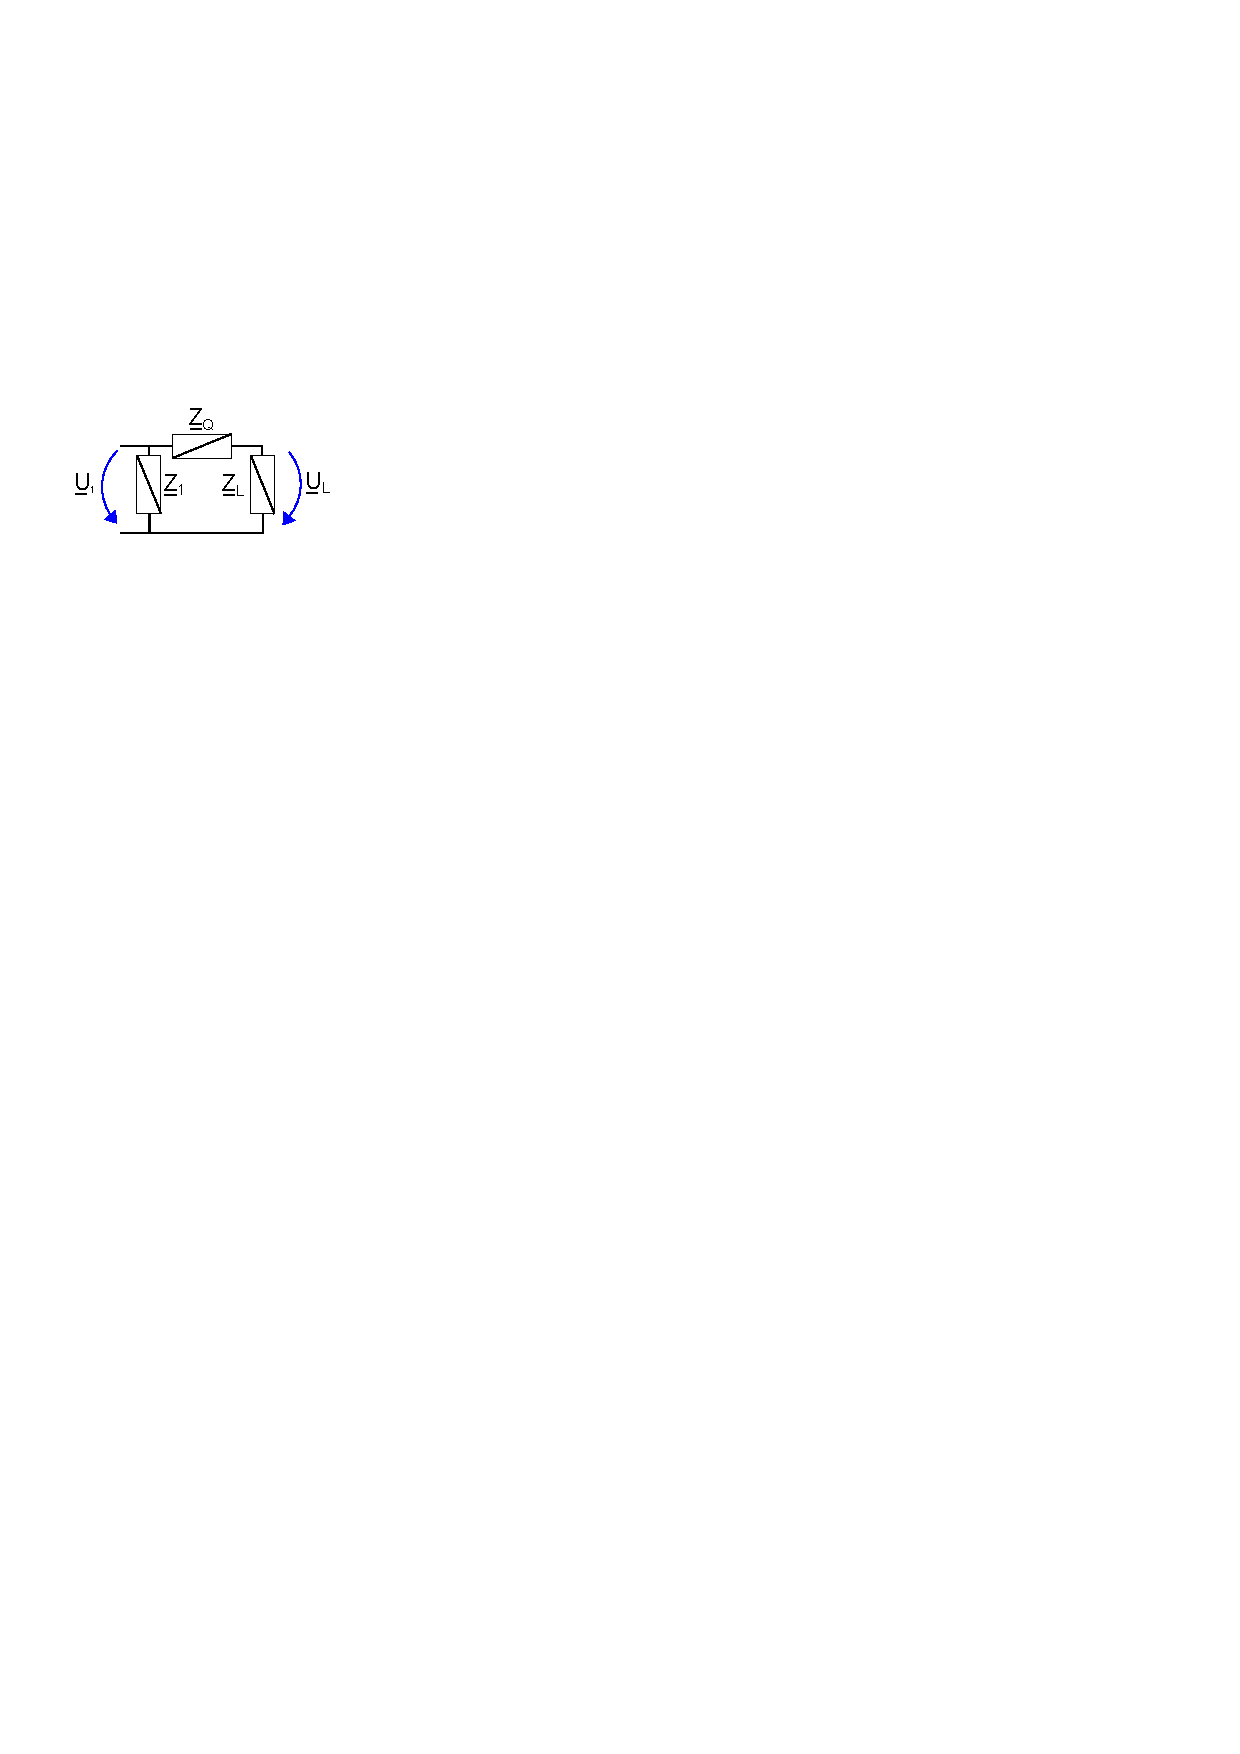
\includegraphics[width=\textwidth]{./images/WechselDrehstromrechnung.pdf}
\end{minipage}
\begin{minipage}[rt]{9cm}
	\begin{equation*}
		\underline{U}_L = \frac{\underline{Z}_L}{\underline{Z}_L + \underline{Z}_Q} \cdot \underline{U}_1
	\end{equation*}
\end{minipage}
  
\section{Grundlagen Drehfeldmaschinen}
    \subsubsection{Stern- (Y) / Dreieckschaltung ($\Delta$)}
        \renewcommand{\arraystretch}{2}
        \begin{tabular}{| p{4.5cm} | l | l |}
            \hline
            &
            Sternschaltung (Y) &
            Dreieckschaltung ($\Delta$) \\
            \hline
            \vspace{0.2cm} &
            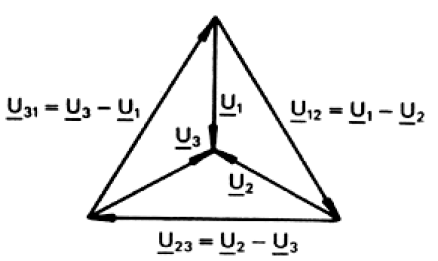
\includegraphics[width=5cm]{images/Sternspannung.png} &
            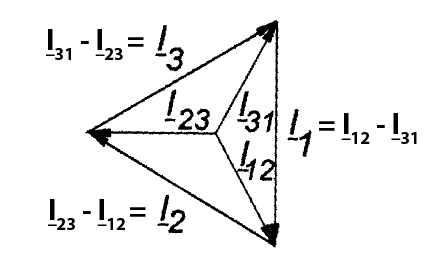
\includegraphics[width=5cm]{images/Dreieckstrom.png} \\
            \hline
            Verkettete Spannung &
            $U = U_{Str} \cdot \sqrt{3}$ \hspace{0.2cm} $\underline{U} = \underline{U}_{Str} \cdot \sqrt{3} \cdot e^{j 30^\circ}$ &
            $U = U_{Str}$ \hspace{0.2cm} $\underline{U} = \underline{U}_{Str}$ \\
            \hline
            Aussenleiterströme &
            $I = I_{Str}$ \hspace{0.2cm} $\underline{I} = \underline{I}_{Str}$ &
            $I = I_{Str} \cdot \sqrt{3} $ \hspace{0.2cm} $\underline{I} = \underline{I}_{Str} \cdot \sqrt{3} \cdot e^{-j 30^\circ} $ \\
            \hline
            Gesamt-Scheinleistung &
            $S = 3 \cdot S_{Str} =\sqrt{3} \cdot U \cdot I $ \hspace{0.2cm} in $[VA]$ &
            $S = 3 \cdot S_{Str} = \sqrt{3} \cdot U \cdot I$ \hspace{0.2cm} in $[VA]$ \\
            \hline
            Scheinleistung pro Strang &
            \multicolumn{2}{l|}{\hspace{3cm} $S_{Str} = U_{Str} \cdot I_{Str}$ \hspace{0.2cm} in $[VA]$} \\
            \hline
            Wirkleistung &
            \multicolumn{2}{l|}{\hspace{3cm} $P = S \cdot \cos\varphi = \sqrt{3} \cdot U \cdot I \cdot \cos\varphi$ \hspace{0.2cm} in $[W]$} \\
            \hline
            Blindleistung &
            \multicolumn{2}{l|}{\hspace{3cm} $Q = S \cdot \sin\varphi = \sqrt{3} \cdot U \cdot I \cdot \sin\varphi$ \hspace{0.2cm} in $[var]$} \\
            \hline
        \end{tabular}
        \renewcommand{\arraystretch}{1.5}

    \subsubsection{Stern-Dreieck-Umwandlung}
        \begin{minipage}[lt]{7.5 cm}
            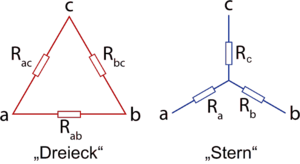
\includegraphics[width=6cm]{images/stern-dreieck.png}
        \end{minipage}
        \begin{minipage}[rt]{9.35 cm} %BASTEL!!
            \renewcommand{\arraystretch}{2}
            \begin{tabular}{ll}
                Umwandlung $\triangle \rightarrow Y$: &
                $Z_{c} = \dfrac{Z_{ac} Z_{bc}}{Z_{ab}+Z_{bc}+Z_{ac}}$ \\
                & $I_{ab} = \frac{I_a \cdot Z_a - I_b \cdot Z_b}{Z_{ab}}$ \\
\                Umwandlung $Y \rightarrow \triangle$: &
                $Y_{ac}=\dfrac{Y_{a} Y_{c}}{Y_{a}+Y_{b}+Y_{c}}$ \\
                Bei gleichen Widerständen: &
                $R_Y = \frac{R_\triangle}{3}$ \\
                Bei gleichen Kapazitäten: &
                $C_Y = C_\triangle \cdot 3 $ \\
                Bei gleichen Induktivitäten: &
                $L_Y = \frac{L_\triangle}{3}$
            \end{tabular}
            \renewcommand{\arraystretch}{1.5}
        \end{minipage}
       
\section{Drehstrom- Synchronmaschinen(DSM)}
%    \subsection{Aufbau der DSM}
%        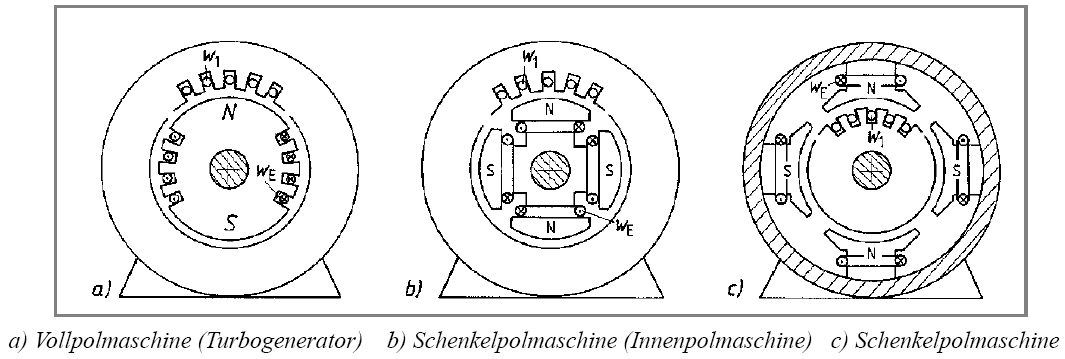
\includegraphics[width=12cm]{./images/Aufbau_DSM.png}\\
%        \begin{description}
%            \item[Innenpolmaschine:] Der Läufer ist ein Dauermagnet, oder wird mit Gleichstrom und über Schleifer
%            zu einem solchem gemacht. Dieser läuft mit dem aussen anliegendem Drehfeld mit.
%            \item[Aussenpolmaschine:] Der Läufer erzeugt ein Drehfeld, welches sich immer am konstanten Statorfeld
%            ausrichtet. Worauf sich des Läufer dreht.
%            \item[Turbomaschine:] Die Schleiferlose Variante. Mit Hilfe eines Hilfsgenerator auf der gleichen Welle
%            wird ein Drehstrom erzeugt, welcher auf dem Läufer selbst gleichgerichtet wird. Damit wird dan ein
%            konstantes Magnetfeld (Dauermagnet) erzeugt (wie die Innenpolmaschine).
%        \end{description}
    \subsection{Ersatzschaltbild}
        \begin{minipage}{11cm}
            \abb{images/Ersatz_DSM.png}{8cm}{Ersatzschaltung DSM}    
            Es gibt 2 Unterteilungen:
            \begin{description}
                \item[Wirkleistung:] Gibt die DSM leistung ab oder nimmt sie auf. Zu erkennen ist das am Phasenwinkel
                zwischen $U_{KL}$ und $U_P$. Ist $U_P$ voreilend, so ist es ein \textbf{Generator}, anderseits ein
                \textbf{Motor}.
                \item[Blindleistung:] Blindleistung Auf- oder Abgabe. Bei \textbf{Übererregung} oder auch \textbf{kapazitiven
                Betrieb} gibt der DSM Blindleistung ab. Bei \textbf{Untererregung} oder auch \textbf{induktiven Betrieb}
                nimmt er auf.
            \end{description}
        \end{minipage}
        \begin{minipage}{8cm}
      %      \abb{images/Zeigerdiagram.png}{6cm}{Betriebszustände einer DSM}
    	  	\subsubsection{Phasenschieber}
	      	Ein DSG, der im Idealfall nur Blindleistung mit dem Netz austauscht. In der Praxis müssen die Verluste des DSG(Reibung, Ventilation, Stromwärme etc.) entweder vom Netz oder von einer Antriebsmaschine gedeckt werden.
			Der Phasenschieber kennt folgende Betriebsmodi:
     		\begin{itemize}
     			\item \textbf{\emph{übererregt}} $(U_p > U_N)$: der DSG gibt Blindleistung ab, verhält sich also bezüglich seiner Klemmen wie ein Kondensator.
      			\item \textbf{\emph{untererregt}} $(U_p > U_N)$: der DSG nimmt Blindleistung auf, verhält sich also bezüglich seiner Klemmen wie eine Induktivität.
      		\end{itemize}
        \end{minipage}
        \begin{minipage}[lt]{10cm}
        	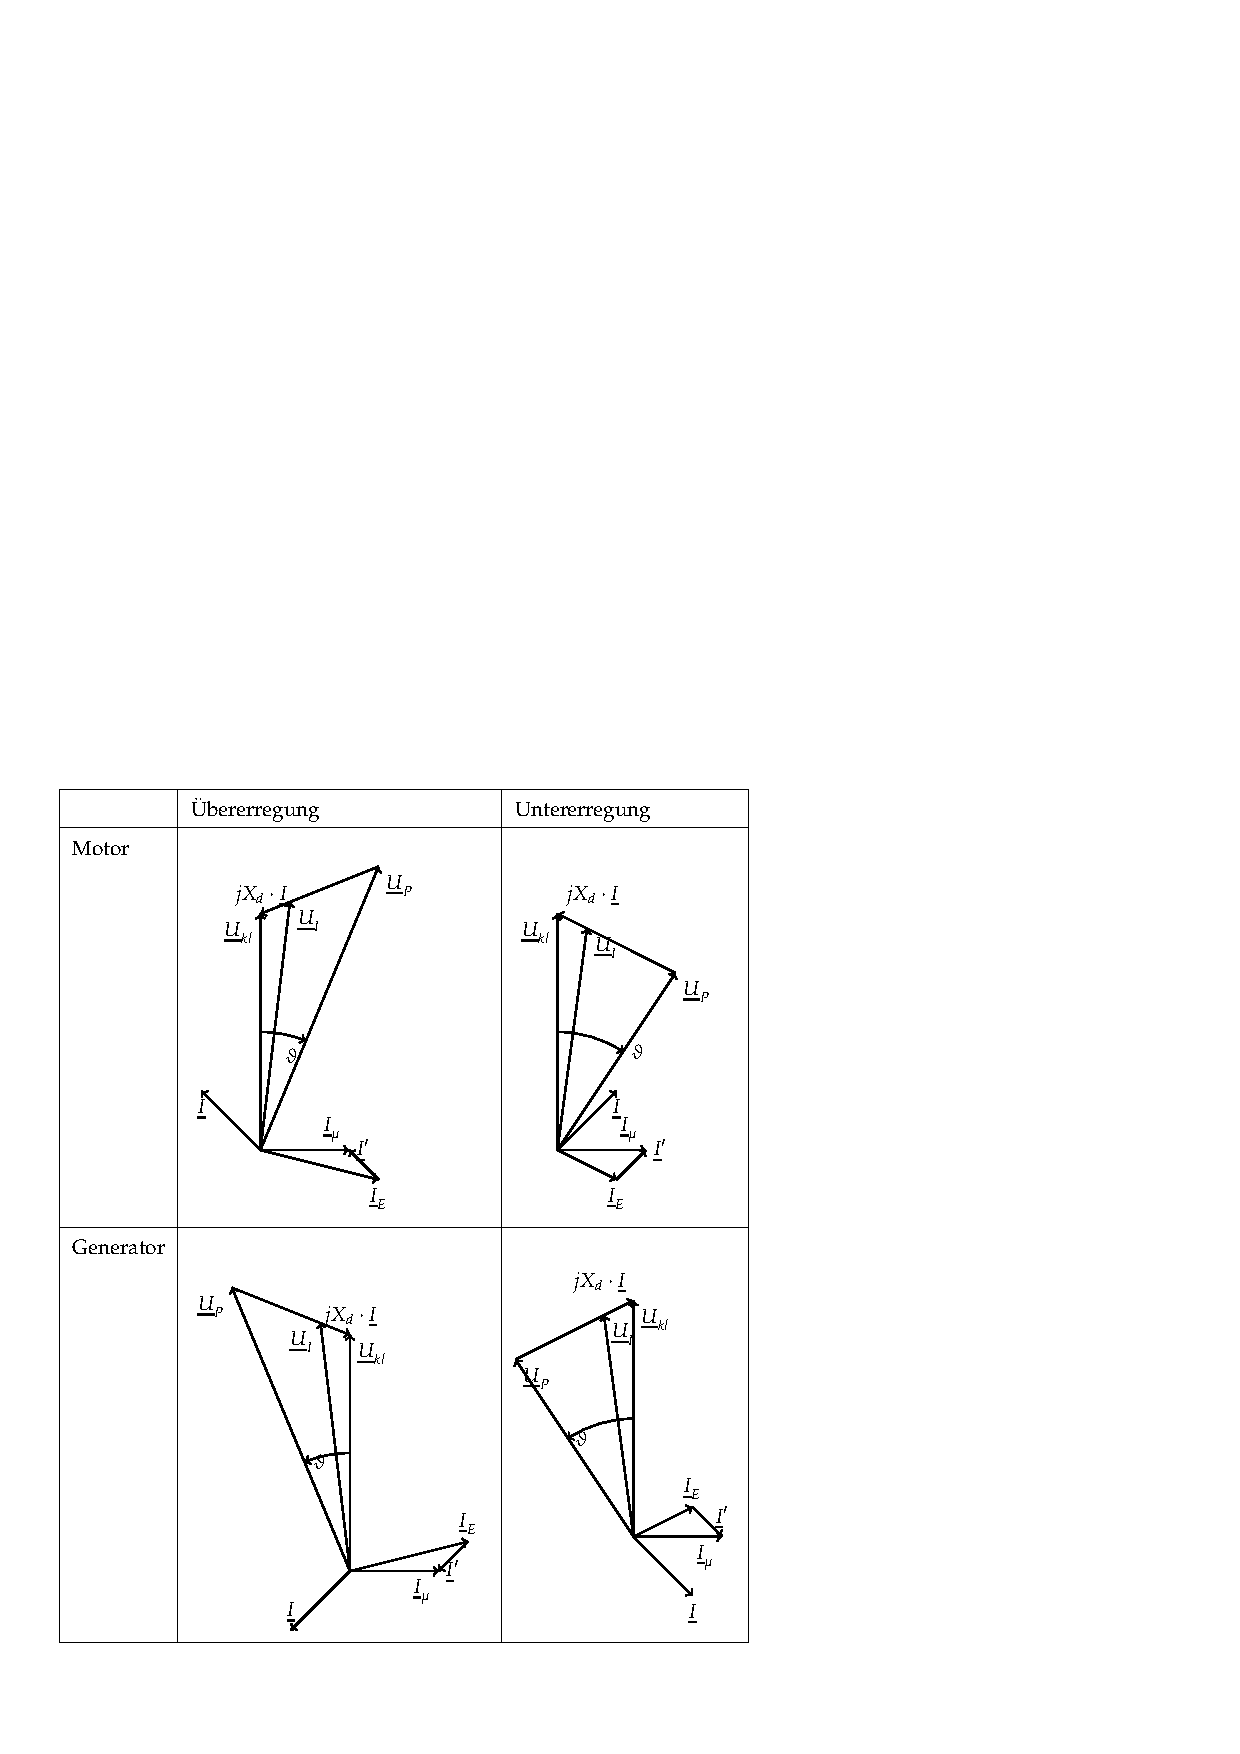
\includegraphics[width=0.8\textwidth]{./images/Zeiger.pdf}
        \end{minipage}
        \begin{minipage}[rt]{8cm}
        	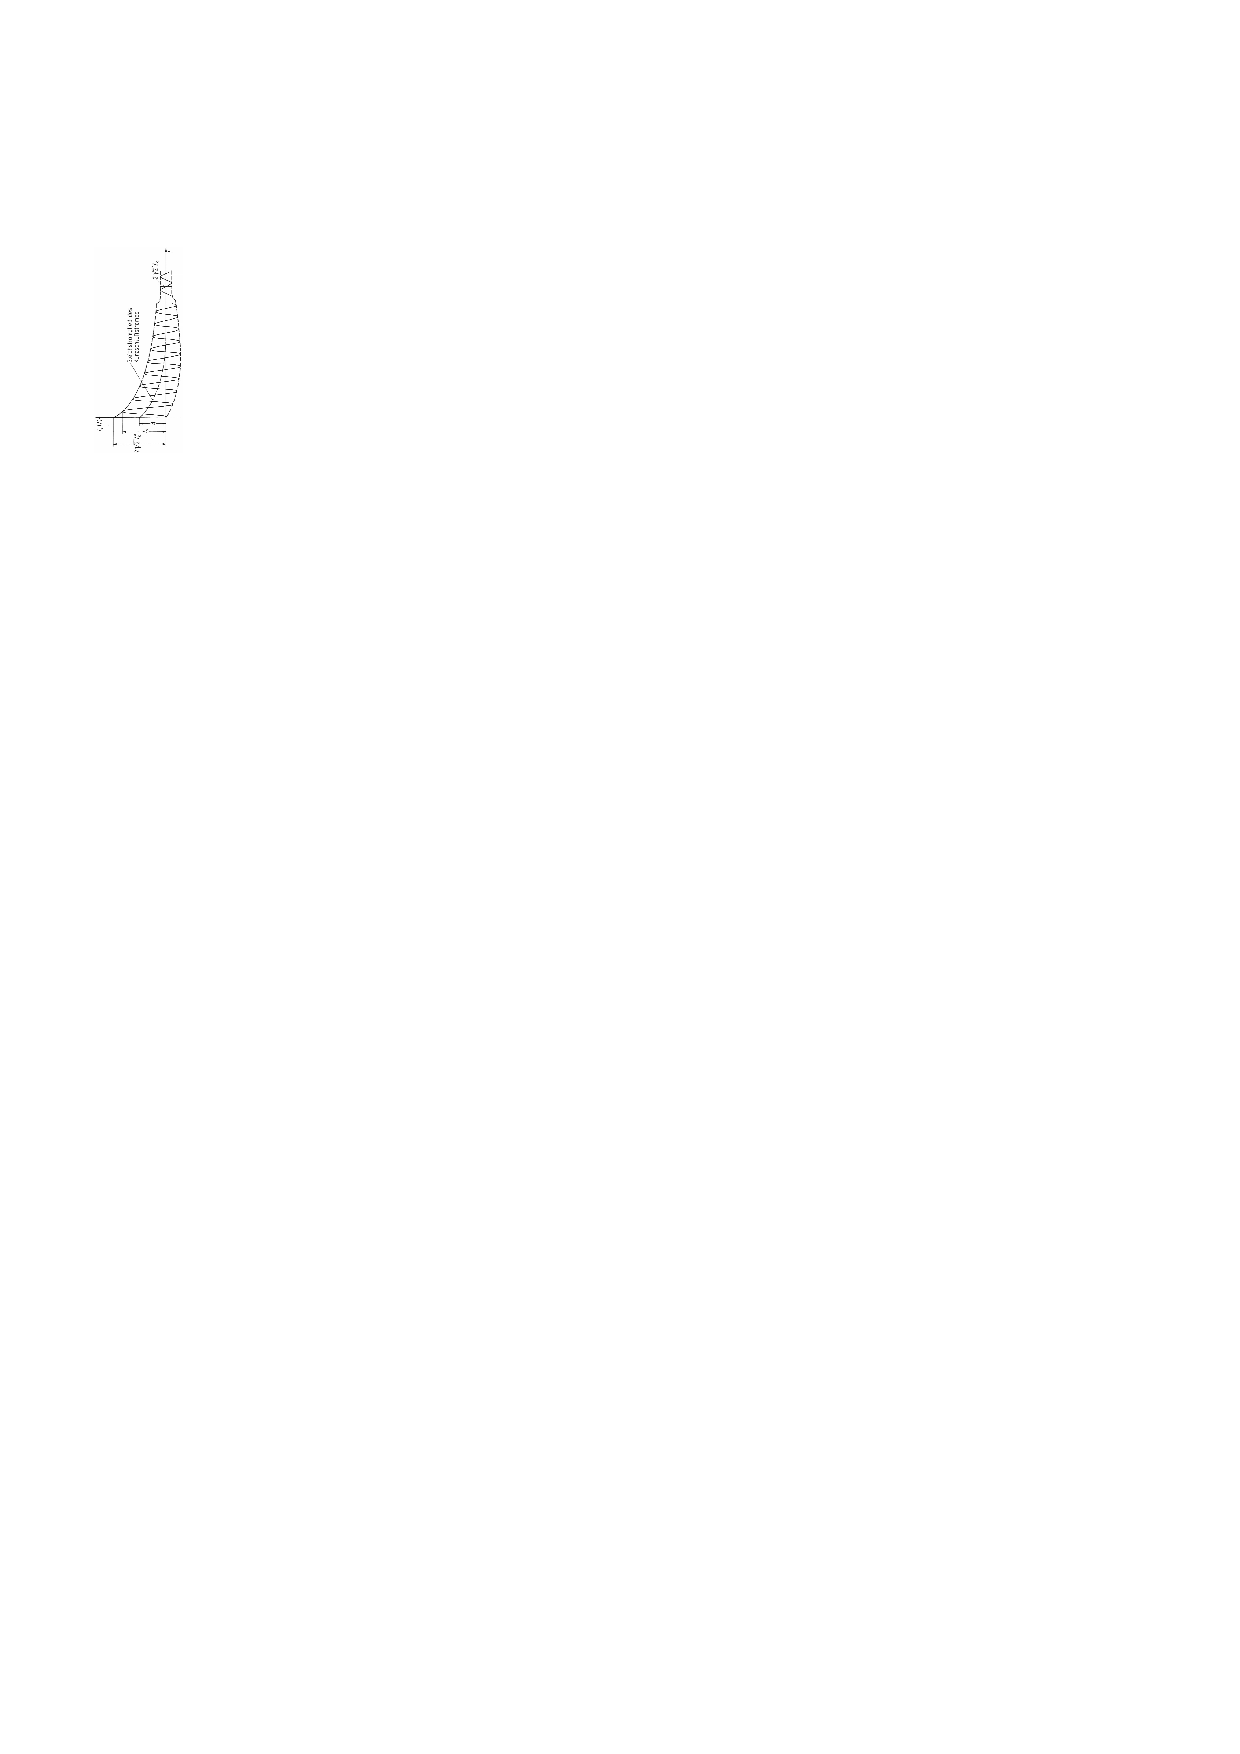
\includegraphics[width=0.4\textwidth]{./images/SM_SC.pdf}
        	\label{SM_SC}
        	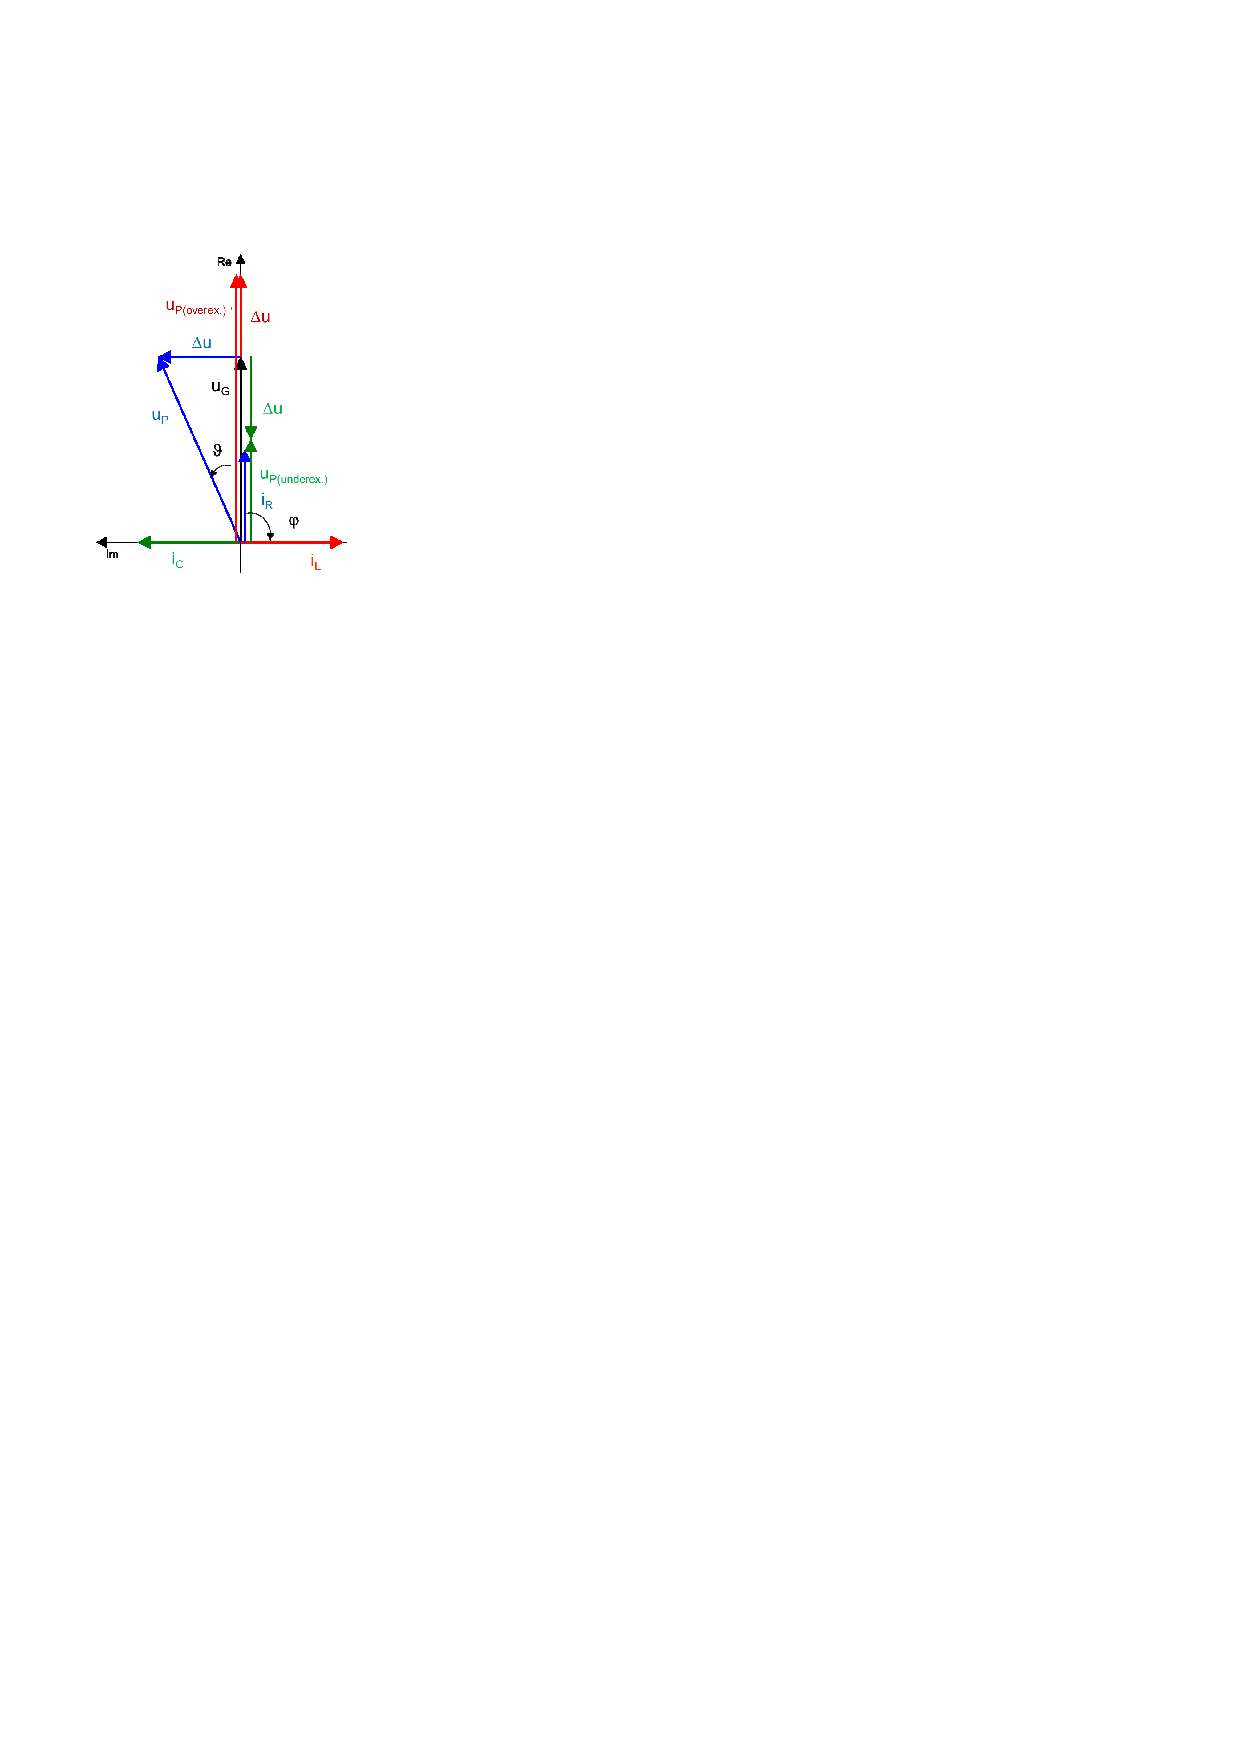
\includegraphics[width=0.6\textwidth]{./images/SM_load.pdf}
        	\label{SM_load}
        \end{minipage}
        
    \subsection{Allgemeine Formeln}
    \begin{longtable}[c]{ | p{6.5cm} | p{11.5cm} |} 
    	\hline
    	Polpaarzahl	& $p$\\
    	\hline
    	Drehfeldzahl $[s^{-1}]$ bzw $[min^{-1}]$ & $n =\frac{f}{p}$ bzw
    	$n =\frac{f\cdot 60}{p}$\\
    	\hline
    	Schlupf $[-]$ & $s=\frac{n_d-n}{n_d}$\\
    	\hline
    	Spannungsfall über Synchroner Reaktanz & $\underline{U}_{X_D}=jX_d\cdot\underline{I}$
    	\\
    	\hline
    	Leerlauferregerstrom für Nennspannung & $I_{E0N}$\\
    	\hline
    	Lastabhängiger Erregerstrom & $\frac{I_{Eneu}}{I_{Ealt}}=\frac{U_{Pneu}}{U_{Palt}}$(im Leerlauf ist $U_p = U_{Kl}$)\\
    	\hline
    	Klemmenspannung & $U_{kl} = \frac{U_N}{\sqrt{3}}$\\
    	\hline
    	Strang- bzw. Phasenspannung &
    	$\underline{U}_{kl}=\underline{U}_p+\underline{U}_{X_D}$\\
    	\hline
    	Polradspannung & $U_p=\sqrt{U_{Kl}^2+X_d^2\cdot I^2+2\cdot U_{Kl}\cdot
    	X_d \cdot I\cdot sin \varphi}$\\
    	\hline
    	\multirow{2}{6.5cm}{Elekrischer Lastwinkel oder Polradwinkel  gem. ESB} & $\vartheta = arg(U_p)$ (Winkel zwischen $U_{p}$ und $U_{kl}$)\\ & $|U_P| \cdot sin(\theta) = |U_{XD}| \cdot cos(\Phi)$\\
    	\hline
    	Wirkleistung des DSG & $P_{el}=3\cdot
    	U_{Kl}\cdot\frac{U_p}{X_d}\cdot \sin\vartheta = 3 \cdot U_{Kl} \cdot I \cdot \cos{\varphi} = M \cdot \omega \cdot \eta$\\
    	\hline
    	Wirkkomponente des Statorstroms & $I \cdot \cos{\varphi} = \frac{U_p}{X_d} \cdot \sin{\varphi}$ \\
    	\hline
    	Antriebsmoment des DSG & $\begin{aligned}
    								M_{Welle} 	&=\frac{3\cdot60}{2\pi\cdot n \cdot
    								    				\eta}\cdot U_{Kl}\cdot\frac{U_p}{X_d}\cdot\sin\vartheta
    								    		&= \frac{3\cdot60}{2\pi\cdot n \cdot
    								    	    	\eta}\cdot U_{Kl}\cdot I \cdot \cos{\varphi}= \frac{P_{mech}}{\omega} \\
    								    	    &= \frac{\sqrt{3} \cdot U_N \cdot I_N \cdot cos\varphi_N \cdot p}{\eta \cdot 2 \cdot \pi \cdot f_N} 
    								\end{aligned}$\\
    	\hline
    	Leistung für Turbogeneratoren & $S_N = c \cdot n \cdot D^2 \cdot l_i; \hspace{1cm} c = \frac{\pi^2}{\sqrt{2}} \cdot 0.9 \cdot A \cdot B_\delta \hspace{1cm} A = \frac{p' \cdot number_{phase} \cdot N \cdot I}{D \cdot \pi}$ \\
    	\hline
    	p.u. & $x_d = X_d \frac{I_N}{U_N/\sqrt{3}} = X_d \frac{S_N}{U_N^2}$; $\hspace{1cm}u_{kl} = \frac{U_{kl}}{U_N}$; $\hspace{1cm} i_{kl} = \frac{I_{kl}}{I_N}$ \\
        \hline
        Spannung unter Last (siehe Abb. \ref{SM_load})& $\begin{aligned}
        						\Delta\underline{u} &= \underline{i} \cdot j x_d = \left(i_R - j i_L + j i_C\right) = i_L x_d - i_C x_d + j i_R x_d \\
        						\underline{u}_P &= u_{kl} + \Delta \underline{u} = u_{kl} + i_L x_d - i_C x_d + j i_R x_d 
        					   \end{aligned}$\\
        \hline
    	Short circuit of an SM (siehe Abb. \ref{SM_SC}) \newline $I_k''$: Initial SC AC current  \newline $I_S$: maximal asymmetric SC current \newline $I_k$: continuous SC current \newline $x_d''$: normally 10 times lower than $x_d (0 - 100ms)$, subtransient \newline $x_d'$: is as twice as high than $x_d'' (100 - 500ms)$,  transient \newline $\underline{u}_{0\lambda}, \underline{i}_0: \text{values before SC}$ &
      	$\begin{aligned}
	    	\underline{i}_k(t) &= \left(\underline{i}_k'' - \underline{i}_k'\right) e^{-\frac{t}{T_d''}} + \left(\underline{i}_k' - \underline{i}_k\right) e^{-\frac{t}{T_d'}} + \underline{i}_k\\
	    	\underline{i}_k'' &= \frac{\underline{e}''}{j x_d''} \hspace{1cm}\underline{e}'' = \underline{u}_{0\lambda} + j x_d'' \cdot \underline{i}_0 \approx 1.1 (\textrm{worst case})	\\	
	    	\underline{i}_k' &= \frac{\underline{e}'}{j x_d'} \hspace{1cm} \underline{e}' = \underline{u}_{0\lambda}+ j x_d' \cdot \underline{i}_0 \approx 1.15\\
	    	\underline{i}_k &= \frac{\underline{e}}{j x_d} \hspace{1cm} \underline{e} = \underline{u}_{0\lambda} + j x_d \cdot \underline{i}_0 \\
	     \end{aligned}$ \\
 		\hline
    \end{longtable}
    \label{tab:SM}
    
%    \subsection{Inselnetz}
%    \begin{tabular}{|p{7cm}|p{11cm}|}
%    		\hline
%        	Netzstrom Generator & Verbraucherstrom vom Netz mit Immaginiärteil negiert !\\  
%        	\hline
%        	Zuleitungstrom Generator & Netzstrom mit Winkel $+ 180$\textdegree \\
%        	\hline
%        	Verbraucher induktiv & Generator kapazitiv $=$ übererregt \\
%        	Verbraucher kapazitiv & Generator induktiv $=$ untererregt \\
%        	\hline
%        	Polradspannung & $\underline{U}_p = \underline{U}_{kl} - \underline{U}_{XD} $ \\
%        	\hline
%        	Polradspannung im Inselnetz & $U_p=\sqrt{U_{Kl}^2+X_d^2} $\\
%        	\hline
%        	Klemmenspannung & Y = 230V $\Delta$ = 400V \\
%        	\hline
%        	Klemmenspannung nach Lastabwurf & $U_{Kl} = \sqrt{3} \cdot U_p $\\
%        	\hline
%    \end{tabular}

    \subsection{Betriebsverhalten}
    	Siehe Abbildung \ref{fig:betriebsverhalten}
    	\begin{figure}[h!]
	    	\centering
	    	\begin{subfigure}[t]{0.45\textwidth}
	    		\centering
	    		\adjustbox{scale=0.8}{\begin{tikzpicture}
 	\draw[->] (-0.1,0) -- +(4.6,0) node[below] {I};
 	\draw[->] (0,-0.1) -- +(0,4.6) node[left]{U};
 	\draw (0,0) -- +(4.2,4.2);
	\draw[thick]  plot[smooth, tension=.7] coordinates {(0,0) (1.4,2.4) (4.2,3.4)};
	\draw (5,3.5) node[] {$U = f(I_E)$};
	
	\draw (1.2,0) node[below] {$I'$}
		-- ++(0,1.2) 
		-- ++(-1.2,0) node[left] {$X_h I$};
	\draw (3.16,0) node[below] {$I_\mu = I_{EON}$}
		-- ++(0,3.16) 
		-- ++(-3.16,0) node[left] {$\frac{U_N}{\sqrt{3}}$};
	\draw (4,0) node[above right] {$I_E$}
		-- ++(0,4) 
		-- ++(-4,0) node[left] {$\underline{U}_p$};
	\draw[<-] (3.16,3.16) -- (2,3.4) node[above]{\small{Nennbetriebspunkt}};
\end{tikzpicture}}
	    		\caption{Im Betriebspunkt linearisierte Leerlaufgerade}
	    	\end{subfigure}
	    	\begin{subfigure}[t]{0.45\textwidth}
	    		\centering
	    		\adjustbox{scale=0.8}{\begin{tikzpicture}
 	\draw[->] (-0.1,0) -- +(4.6,0) node[below] {$i_E$};
 	\draw[->] (0,-0.1) -- +(0,4.6) node[left]{$\frac{I_k}{I_N}$};
 	\draw (0,0) -- +(4.2,4.2);
	
	\draw (1.8,0) node[below] {$1$}
		-- ++(0,1.8) 
		-- ++(-1.8,0) node[left] {$i_{k0}$};
	\draw (3.6,0) node[below] {$i_{Ek}$}
		-- ++(0,3.6) 
		-- ++(-3.6,0) node[left] {$1$};
\end{tikzpicture}}
	    		\caption{Kurzschlussgerade}
	        \end{subfigure}
	        \caption{Kurven in den Verschiedenen Betriebsarten}
	        \label{fig:betriebsverhalten}
    	\end{figure}
    	
    	\begin{tabular}{ l l p{9cm} }
    		\textbf{Leerlauf}
    		& $I_E = \frac{U_P \cdot \sqrt{3} \cdot I_{E0N}}{U_N}$ 
    		& Die Formel ist für die liniarisierte Gerade \newline
    		  $I_E: $Erregerstrom \newline
    		  $U_P: $verkettete Nennspannung des DS- Netzes\newline
    		  $I_{E0N}:$Leerlauferregerstrom für Nennspannung
    		\\
    		\textbf{Kurzschluss} 
    		& $X_d=\frac{U_P}{I_{K0}}$
    		& Gilt unter Vernachlässigung des Wicklungswiderstand \newline
    		  Die Kurzschlussgerade ist linear
    		\\
    	\end{tabular} 
    	

%    \subsubsection{Inselbetrieb}
%        \begin{minipage}{10cm}
%            \abb{images/Belastungskennlinie_DSM.png}{9cm}{Belastungskennlinie bei konst. Erregerstrom}
%        \end{minipage}
%        \begin{minipage}{6cm}
%            \abb{images/Regulierungslinie_DSM.png}{6cm}{Regulierungskennlinie für konst. $U_{Kl}$}
%        \end{minipage} \\
%        Die Klemmenspannung nimmt bei kapazitiven Lasten zu, bei induktiven stark ab. Für eine konstante $U_{Kl}$ muss der Erregerstrom wie die Regulierungskennlinie angepasst werden.

    \subsubsection{Netzbetrieb}
        Im Netzbetrieb wird die Frequenz, Klemmenspannung, Umlaufsinn und Phasenlage vom Netz vorgegeben. Das heisst bevor man mit einer DSM ans Netz will, muss man sie so synchronisieren, dass alle jene Parameter mit dem Netz überreinstimmen. Sind die Maschine und Netz synchronisiert und zusammengeschaltet, kann mit Hilfe von $I_E$ und der mechanischen Leistung der Blindstromanteil eingestellt werden: \\
        \begin{minipage}{8.2cm}
            \abb{images/Ortskurve_DSM.png}{8cm}{Ortskurve einer DSM im starren Netz}
        \end{minipage}
        \begin{minipage}{9.7cm}
            \begin{itemize}
                \item Da $U_{Kl} = U_1$ konstant ist, ist der Ursprung des Zeigers $\frac{j \cdot U_p}{X_d}$ immer am gleichen Ort. 
                \item Mit dem Erregerstrom kann man die Länge des Zeigers $\frac{j \cdot U_p}{X_d}$ einstellen.
                \item Die mechanische Leistung ist proportional zum Abstand der Zeigerspitze zur Imaginärachse.
                \item Die Blindleistung ist proportional zum Abstand  der Zeigerspitze zur Reelenachse.
                \item Ist nun die mechanische Leistung konstant und man ändert den Erregerstrom, so wandert die Zeiger auf einer Linie parallel zur Imag-Achse hin und her.
                \item Überschreitet der Zeiger die Stabilitätslinie, schlipft der Läufer durchund es gibt grosse Lärm- und Wärmeentwicklung, da die mechanische Leistung zu gross wird für den Erregerstrom.
                \item Bleibt der Erregerstrom konstant und die mechanische Leistung ändert sich, so wandert der Zeiger auf dem Kreis um (0,$\frac{U_Kl}{j \cdot X_d}$). Jedoch wiederum nur bis zur Stabilitätsgrenze, da dort die Wirkleistung für diesen Erregerstrom maximal ist.
            \end{itemize}
        \end{minipage}
       
\section{Netze}
	\subsection{Komponenten und Technologie von Stromnetzen}
		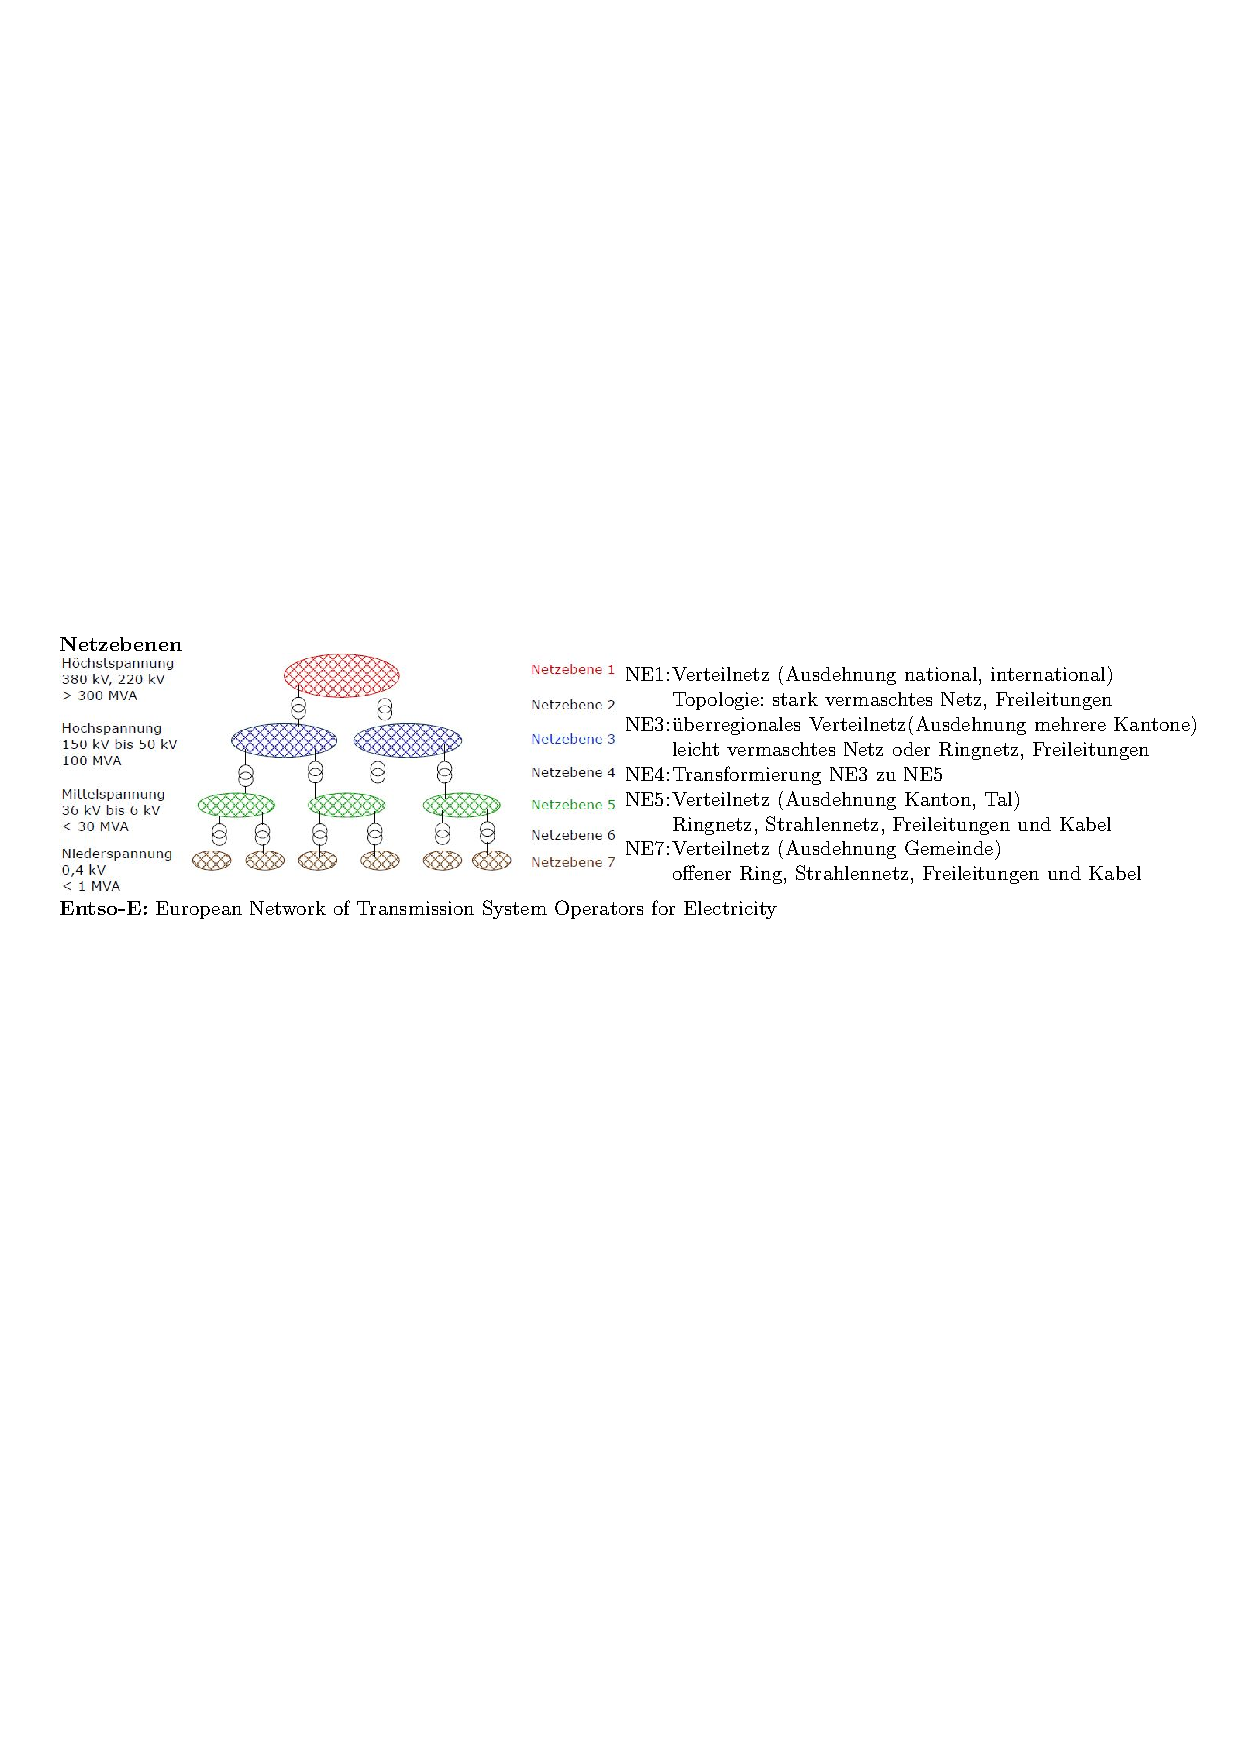
\includegraphics[width=\textwidth]{./images/Netztopologie.pdf}
		
	\subsection{Leitungsbeläge}
	\begin{multicols}{2}
		\textbf{Widerstandsbelag}\\
		Ursache: ohmscher Widerstand des Leiters \\
		$R' = \sigma \frac{\rho}{A}$, $R'$ in $\Omega/m$ \\
		$\sigma$: Verseilfaktor $\left(\sigma \approx 1.07\right)$, $\rho$: Leitungsfähigkeit in $\Omega mm^2/m$, \\
		$A$: Leiterquerschnitt in $mm^2$, $k_{SR}$: Skineffekt \\
		
		\textbf{Induktivitätsbelag}\\
		Ursache: Verkettung der magnetischen Flüsse \\
		$L' = 2 \cdot 10^{-7} \cdot \left(\ln \frac{d}{r_{eq}} + \frac{1}{4}\right) \hspace{1cm} d = \sqrt[3]{d_{12}d_{23}d_{31}}$ \\
		$r$: Leiterradius in $m$, $d$: mittlerer Leiterabstand in $m$ \\
		$d_{ij}$: Abstand zwischen Phase $i$ und $j$ \\
		
		\textbf{Ableitbelag} \\
		Ursache: Korona- und Kriechstromverluste an der Oberfläche\\
		$G'$ in $S/m \Rightarrow$ kann in vielen Fällen vernachlässigt werden\\ \\
		
		\textbf{Kapazitätsbelag}\\
		Überlagerung der Einzelspannungen liefert den Kapazitätsbelag $C'$ in $F/m$ \\
		$C' = \frac{2\pi \epsilon}{\ln \frac{d}{r_{eq}}}$\\
		$r$: Leirerradius in $m$ \\
		$d$: mittlerer Leiterabstand in $m$ \\ 
	\end{multicols}
	\textbf{Bündelleiter}\\
		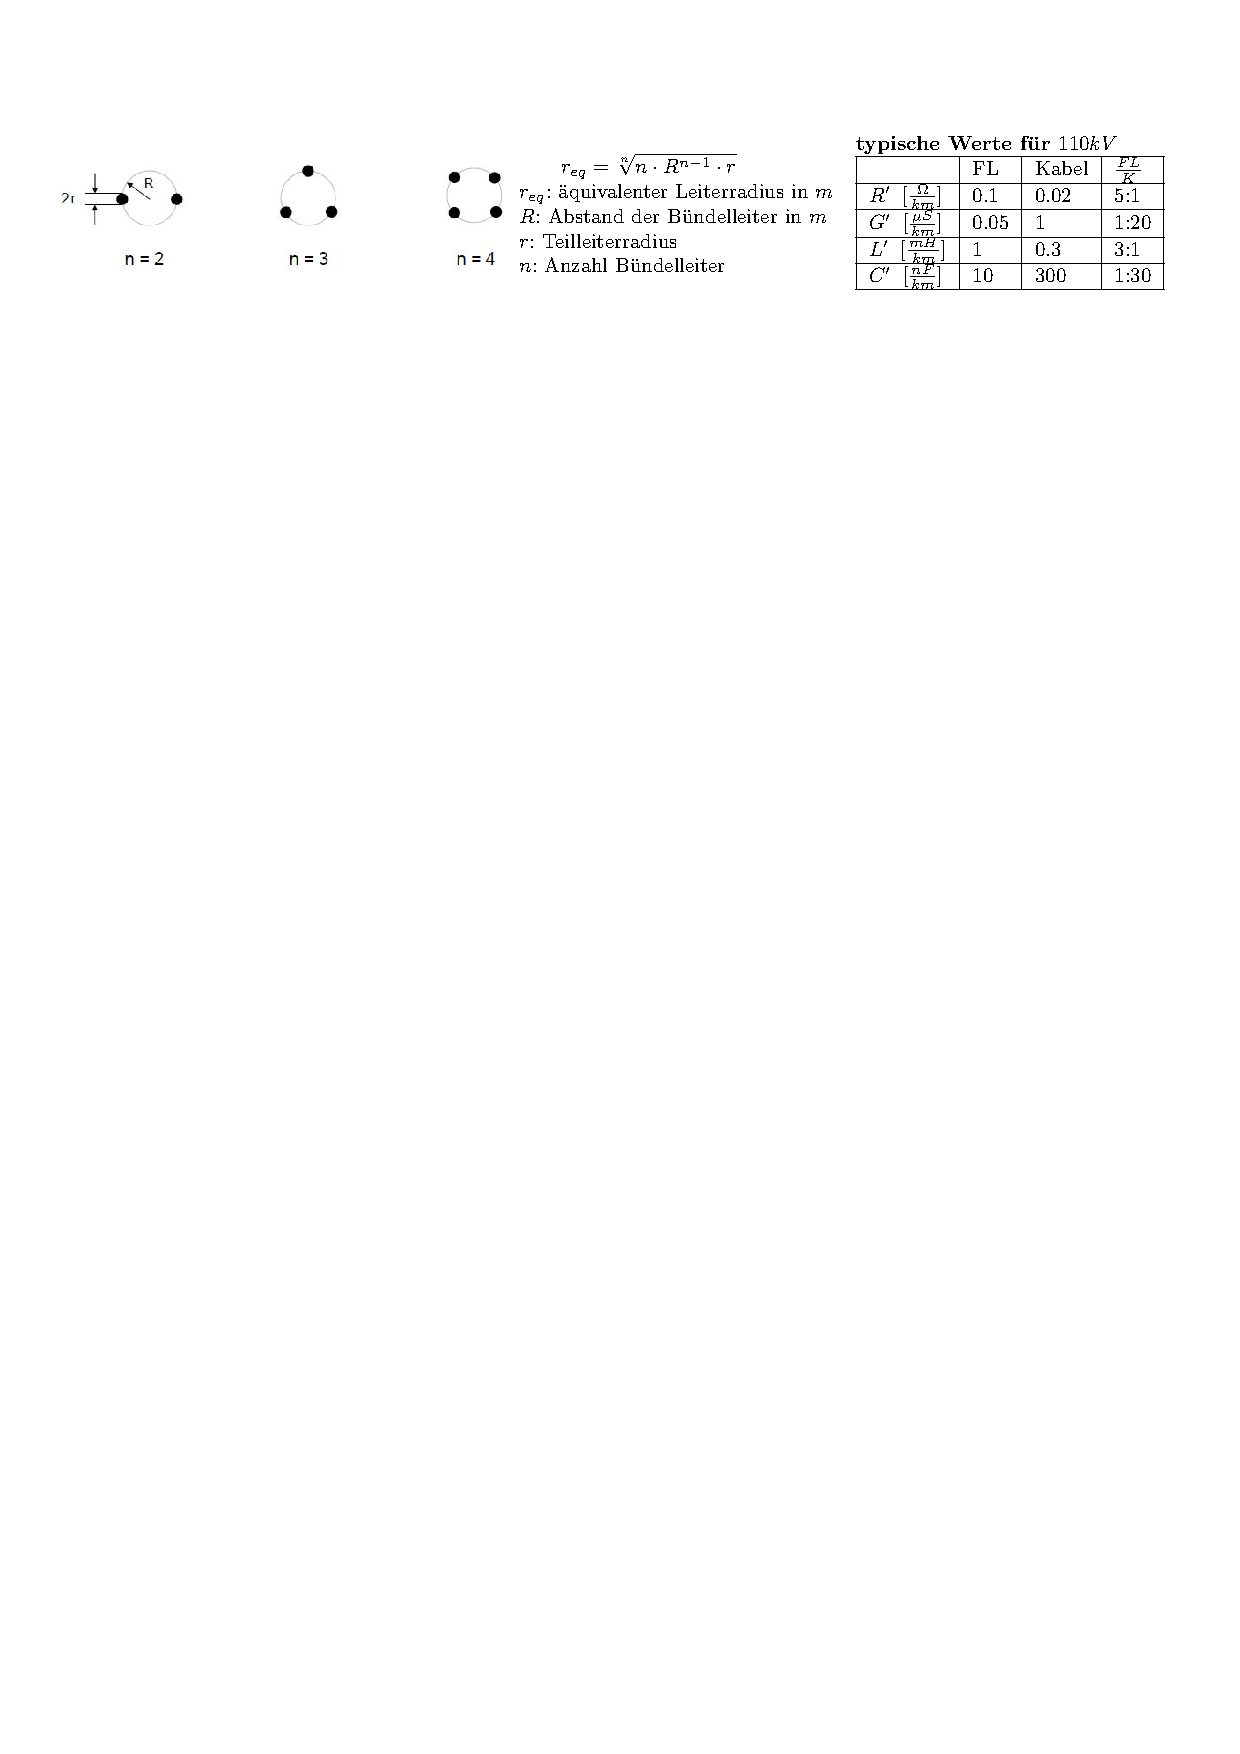
\includegraphics[width=\textwidth]{./images/Buendel.pdf}
	\begin{multicols}{2}
		\textbf{Sag} \\
		\begin{minipage}[lt]{5cm}
			\centering
			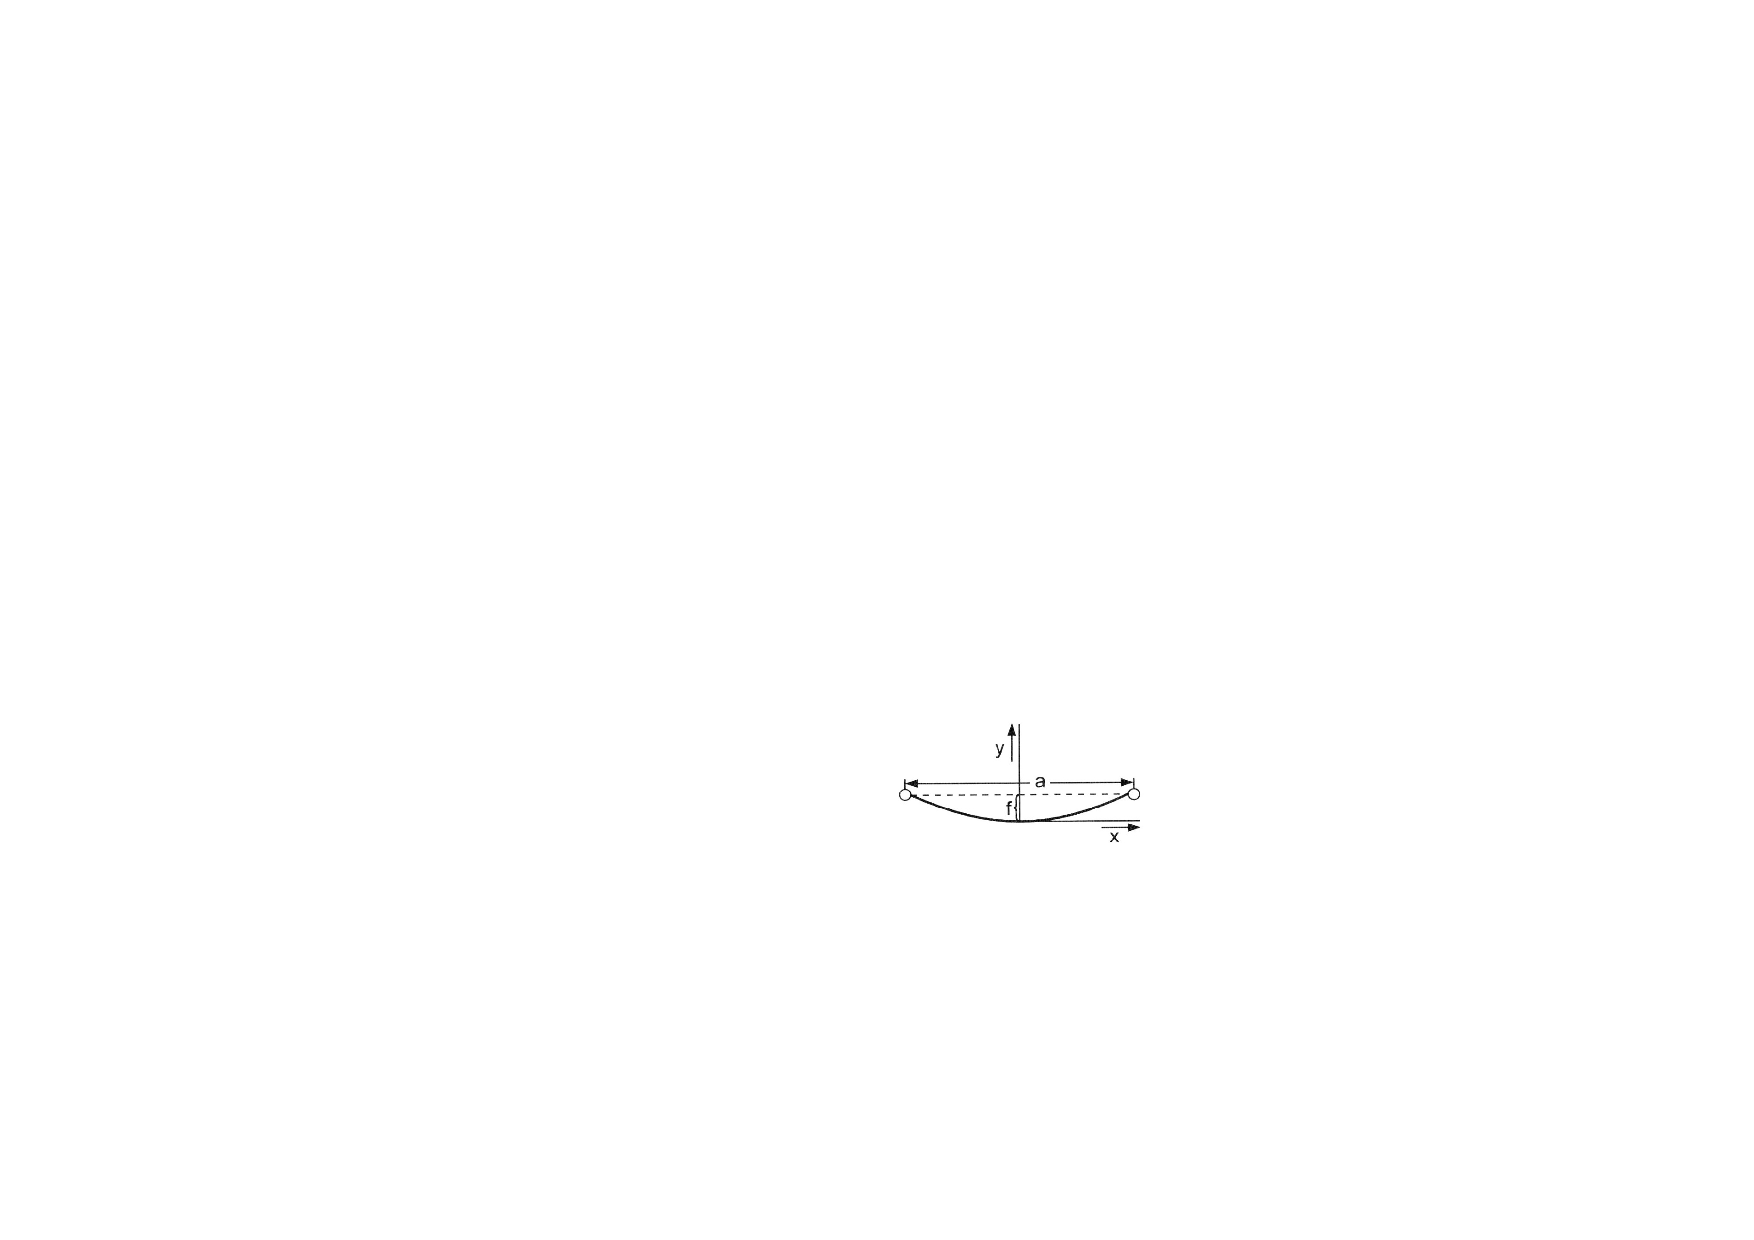
\includegraphics[width=0.7\textwidth]{./images/sag.pdf}
		\end{minipage}
		\begin{minipage}[rt]{5cm}
			$y \approx \frac{mg}{2\sigma}x^2$ \\
			$f_{max} = y \cdot \left(a/2\right)^2$ \\
			$h_{min} = 6 + \frac{U_N - 110~kV}{150~kV}$ 
		\end{minipage}

		\textbf{Skin effect}\\
		{\small $R_\sim = R_= \cdot k_s; \hspace{1cm} k_s \approx 1 + \frac{1}{3}\eta^4$\\
		$ \eta = \frac{r}{2\delta}; \hspace{1cm} \delta = \sqrt{\frac{2\rho}{\omega \cdot \mu}}$ \\
		$R_= = \frac{\rho(\vartheta)\cdot l}{A}; \hspace{1cm} \rho(\vartheta) = \rho_{20} [1+\alpha\left(\vartheta - 20^\circ C\right)]$\\}
	\end{multicols}
		
		
	\subsection{Leitungsmodell und Betriebsverhalten}
		\begin{multicols}{3}
			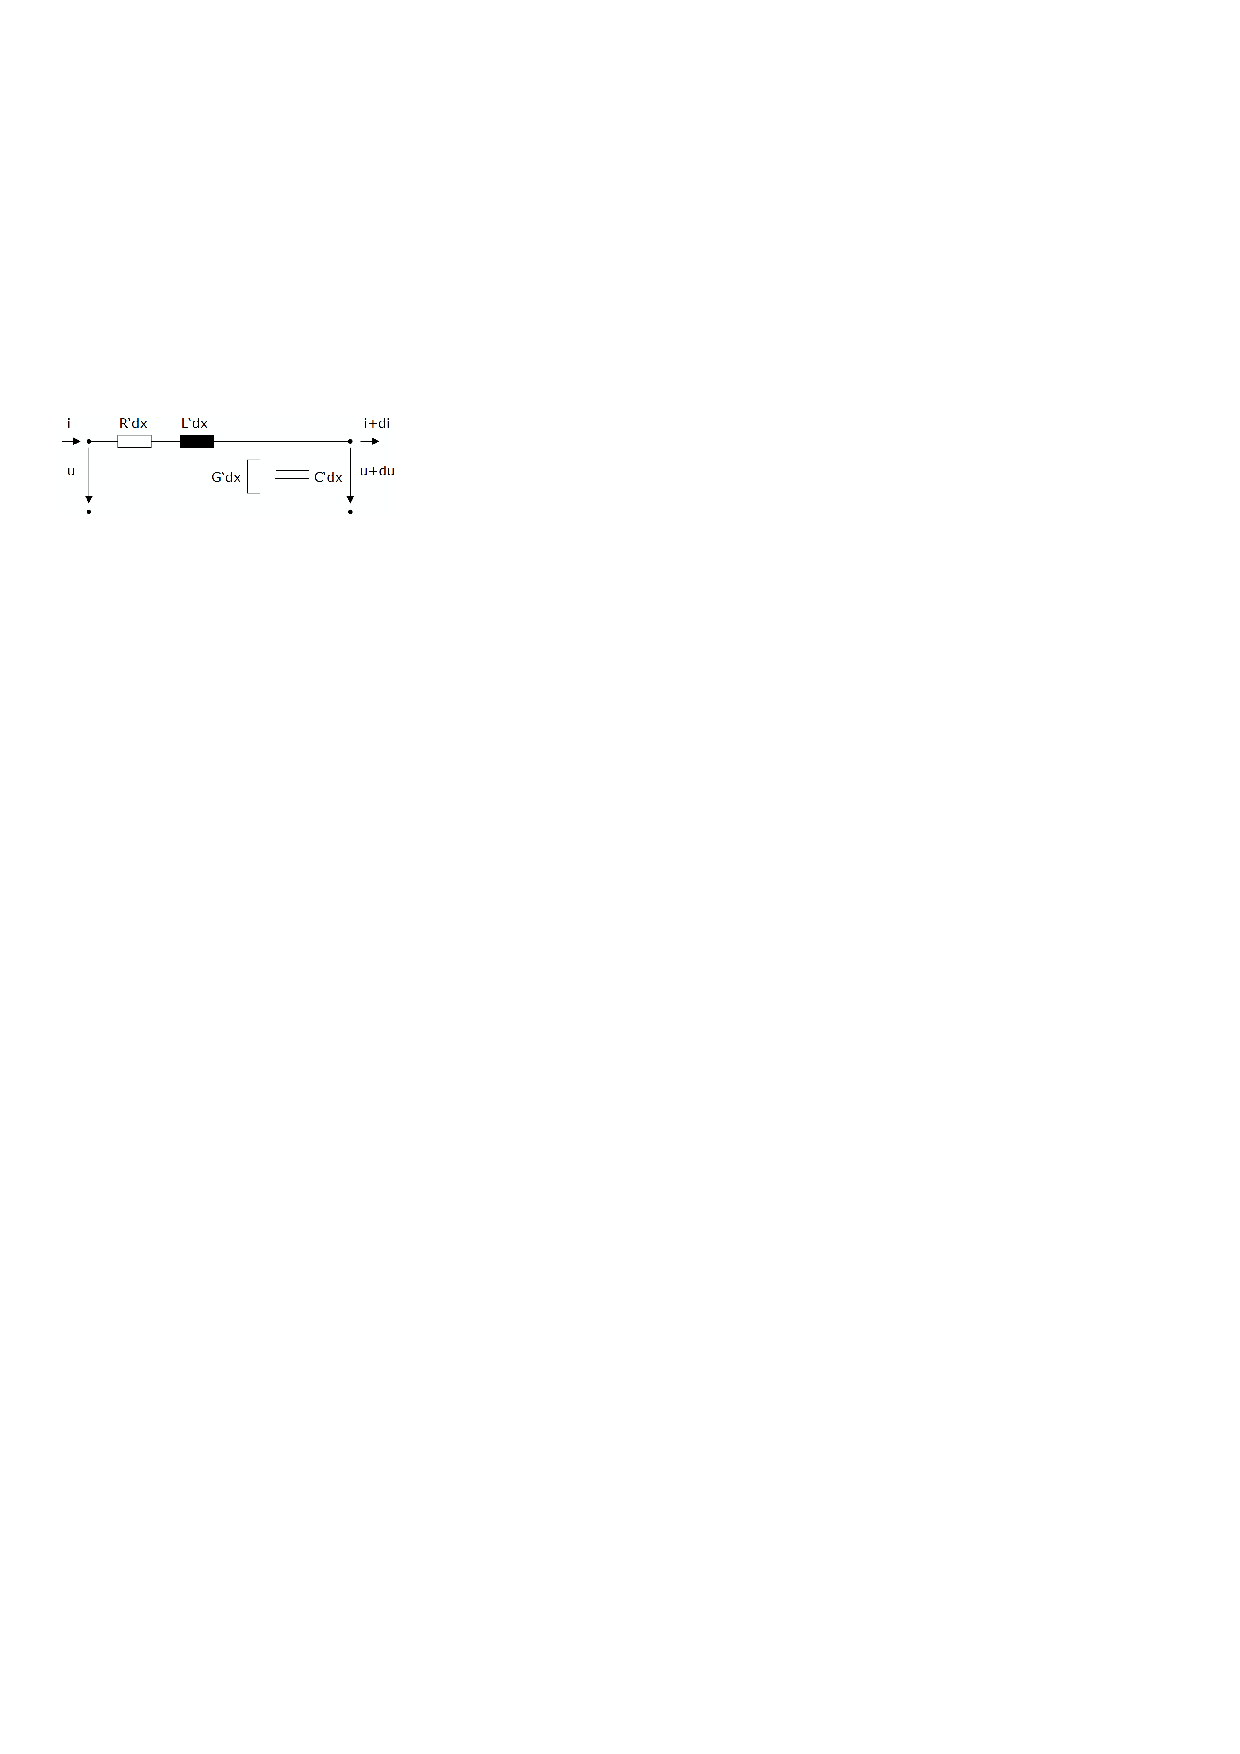
\includegraphics[width=0.28\textwidth]{./images/Leitungsmodell1.pdf} 
			
			allgmeine DGL: \\
			$-du = R'dx \cdot i + L'dx \cdot \frac{di}{dt}$\\
			$-di = G'dx \cdot u + C'dx \cdot \frac{du}{dt}$ \\
			
			DGL für Wechselstrom:\\
			$\frac{d\underline{U}}{dx} = R'\underline{I} + j \omega L' \underline{I}$ \\
			$\frac{d\underline{I}}{dx} = G'\underline{U} + j \omega C' \underline{U}$ 
		\end{multicols}
		Lösung für Wechselstrom:\\
		$\underline{U}_1 = \underline{U}_2 \cosh \underline{\gamma}l + \underline{Z}_w \underline{I}_2 \sinh \underline{\gamma}l \hspace{0.8 cm} \underline{I}_1 = \frac{\underline{U}_2}{\underline{Z}_w} \sinh \underline{\gamma}l + \underline{I}_2 \cosh \underline{\gamma}l \hspace{0.8cm} \underline{\gamma} = \sqrt{\left(R' + j \omega L'\right) \left(G' + j \omega C'\right)}~[\frac{1}{m}] \hspace{0.8cm} \underline{Z}_w = \sqrt{\frac{R' + j\omega L'}{G' + j \omega C'}}~[\Omega]$ \\
		$Z_w \approx \sqrt{X_L X_C} = \frac{1}{2\pi} \sqrt{\frac{\mu_0}{\epsilon_0}} \ln \frac{d}{r} \hspace{1cm}$ \\
		
		\textbf{PI-Ersatzbild (vereinfacht)} \\
		\begin{minipage}[lt]{6cm}
			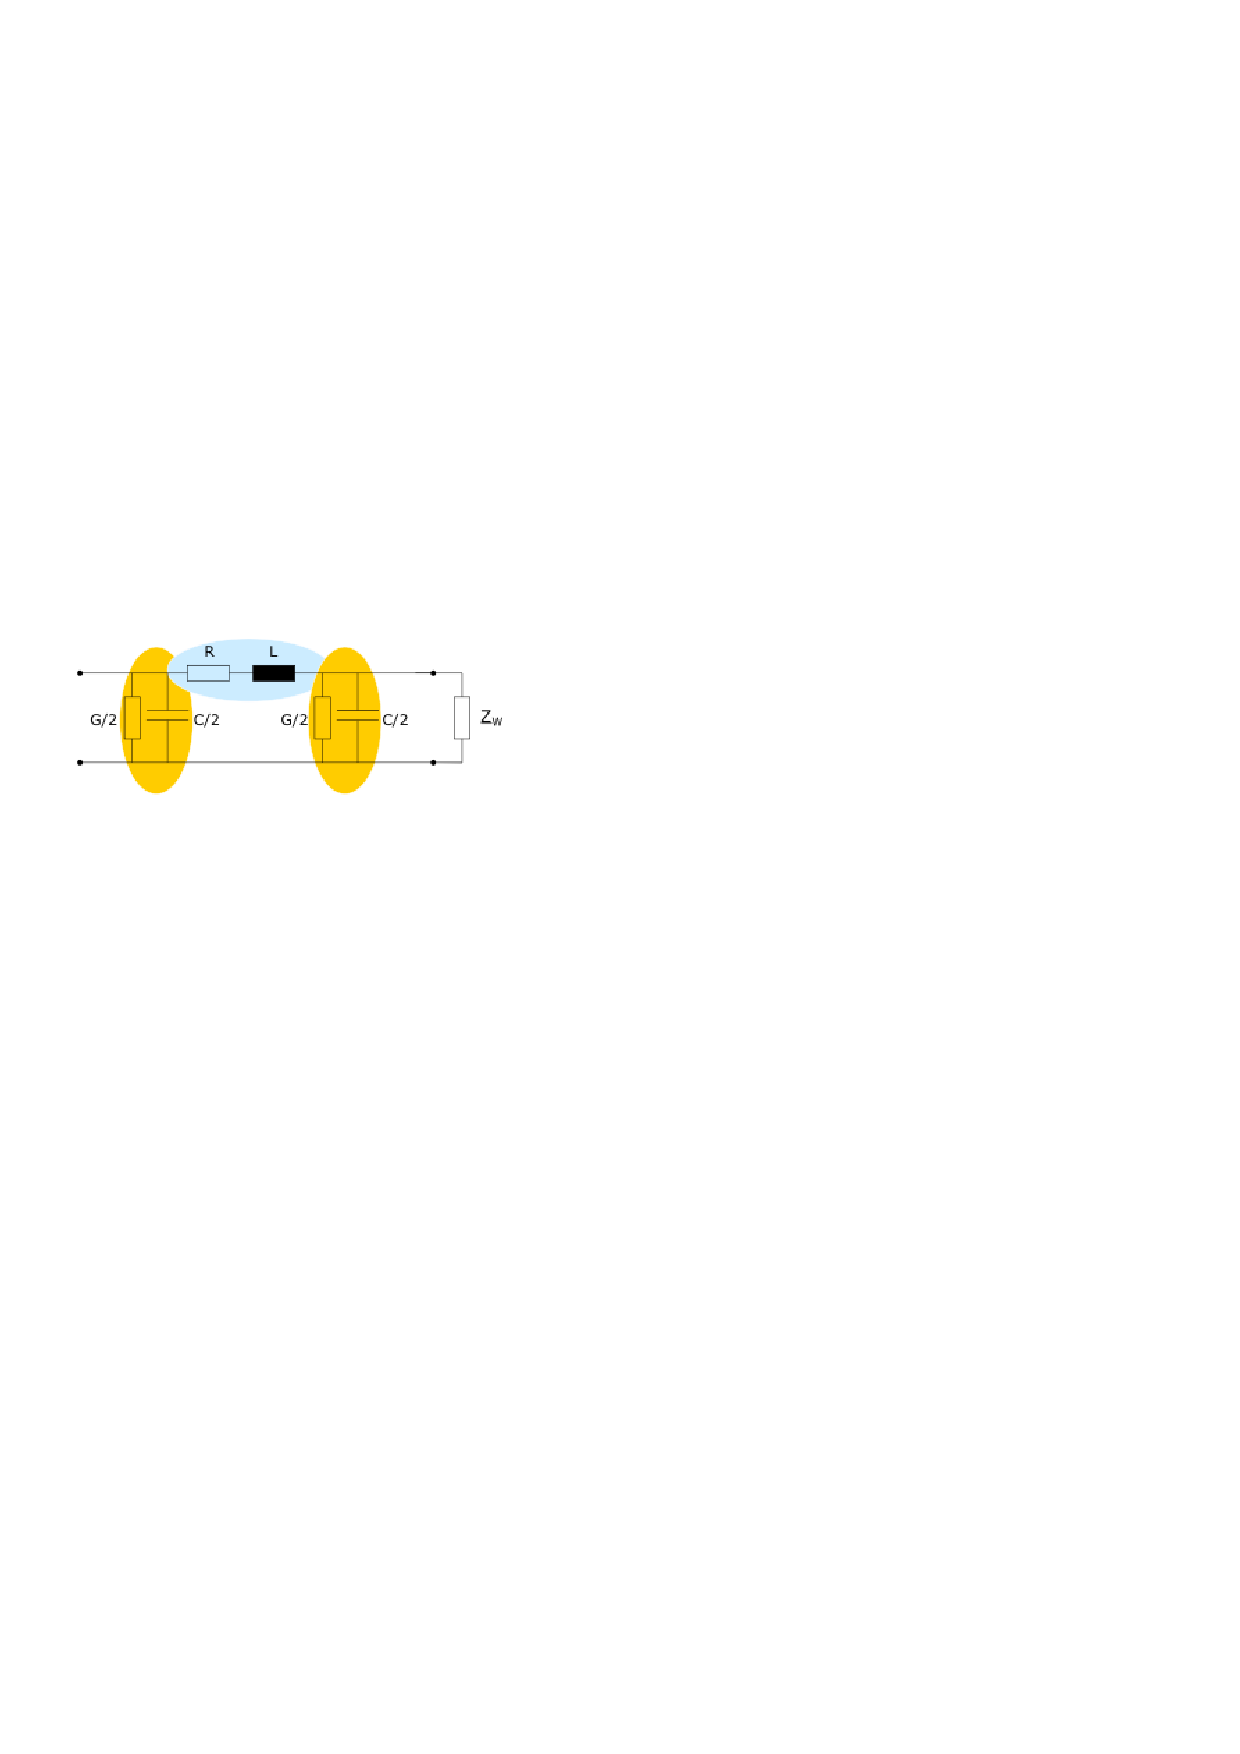
\includegraphics[width=0.9\textwidth]{./images/Leitungsmodell2.pdf}
		\end{minipage}
		\begin{minipage}[rt]{13cm}
			Vereinfachte Modellierung einer Leitung, jedoch nur wenn kürzer als $250~km$(FL)/$50~km$(Kabel) und die Frequenz $50~Hz$ ist. Ersatzbild mit Querimpedanz (gelb) und Längsimpedanz (blau).
		\end{minipage}
		\textbf{Erwärmung der Isolation}: $\tan \delta = \frac{G}{\omega C} \Rightarrow P_V = 3 \cdot U^2 G = U^2 \omega C \cdot \tan \delta$ \\
		\textbf{Spannungsabfall (vereinfacht)}: $\Delta U = \frac{P \cdot R}{U_N} + \frac{Q \cdot X}{U_N}; \hspace{1cm} \Delta u = \frac{\Delta U}{U_N}; \hspace{1cm}$ messen: $\Delta u = \frac{S_A \cdot \cos \varphi}{S_K} \hspace{1cm} \Delta U \approx  \Delta U_L = \sqrt{3} \cdot I \cdot X_L$\\
		\textbf{Relativer Spannungsabfall}: $d = \frac{\Delta U}{U_V} \approx \frac{\Delta S_A}{S_K} \cdot cos(\psi_{K} - \phi) \hspace{1cm}\psi:$ network impedance angle, $\varphi:$ angle of load ($\approx 60^\circ$)\\
		\textbf{Verluste in Leitung}: $P_V = 3 \cdot I^2 \cdot R \hspace{1cm} Q_{ind} = 3 \cdot I^2 \cdot X_L \hspace{1cm} Q_{cap} = \frac{U^2}{X_C} \hspace{1cm} Q_{ges} = Q_{ind} - Q_{cap}$ \\
		\textbf{Ferranti-Effekt}: $\underline{U}_1 = \underline{U}_2 + jX_L \cdot \underline{I}_2; \hspace{1cm} \underline{I}_2 = \frac{\underline{U}_E}{-2jX_C}; \hspace{1cm} \Rightarrow \frac{U_2}{U_1} = \left(1 - \frac{X_L}{2X_C}\right)^{-1} \hspace{1cm} \Delta U = \frac{1}{2} U_1 \omega^2 l^2 C' L'$\\
		
	\subsection{Begriffe}
		\begin{itemize}
				{\small \setlength{\itemsep}{0pt}
				\item \textbf{Kurzschluss}: extreme übernatürliche Belastung, Leitung verhält sich wie $L$, Spannung sinkt entlang der Leitung ab.
				\item \textbf{Leerlauf}: extreme unternatürliche Belastung, Leitung verhält sich wie $C$, $U$-Überhöhung am Leitungsende, Ferranti-Effekt
				\item \textbf{Natürliche Leistung}: Bei einer gewissen Belastung wird in den Querelementen genau so viel Blindleistung erzeugt, wie im Längspfad verbraucht wird. Die Leitung verhält sich neutral bezüglich Blindleistung. Die natürliche Leistung wird übertragen, wenn die Leitung mit $\underline{Z}_w$ belastet wird. $\hspace{1cm} \underline{I}_2 = \frac{\underline{U}_2}{\underline{Z}_w}; \hspace{1cm} \underline{U}_1 = \underline{U}_2 \left(\cosh \underline{\gamma} l + \sinh \underline{\gamma}l\right) = \underline{U}_2e^{\underline{\gamma}l}; \hspace{1cm} I_{nat} = \sqrt{\frac{U_N^2}{3X_LX_C}} = \sqrt{\frac{U_N^2}{3L'/C'}}$
				\item \textbf{Übernat. Belastung}: $\underline{Z}_{Last} < \underline{Z}_w, \underline{Q}_{quer} < \underline{Q}_{laengs}, U$ an Leitungsende ist tiefer als $U$ am Leitungsanfang (KS)
				\item \textbf{Unternat. Belastung}: $\underline{Z}_{Last} > \underline{Z}_w, \underline{Q}_quer > \underline{Q}_{laengs}, U$ an Leitungsende ist höher als $U$ am Leitungsanfang. Freileitungen werden meistens, Kabel immer unternatürlich betrieben (Leerlauf, kapazitiv)
				\item \textbf{Wellenimpedanz}: typische Werte: Freileitungen $\lvert \underline{Z}_w \rvert \approx 300~\Omega$, Kabel $\lvert \underline{Z}_w \rvert \approx 40~\Omega$
				}
		\end{itemize}	
	\subsection{Transformatormodell}
		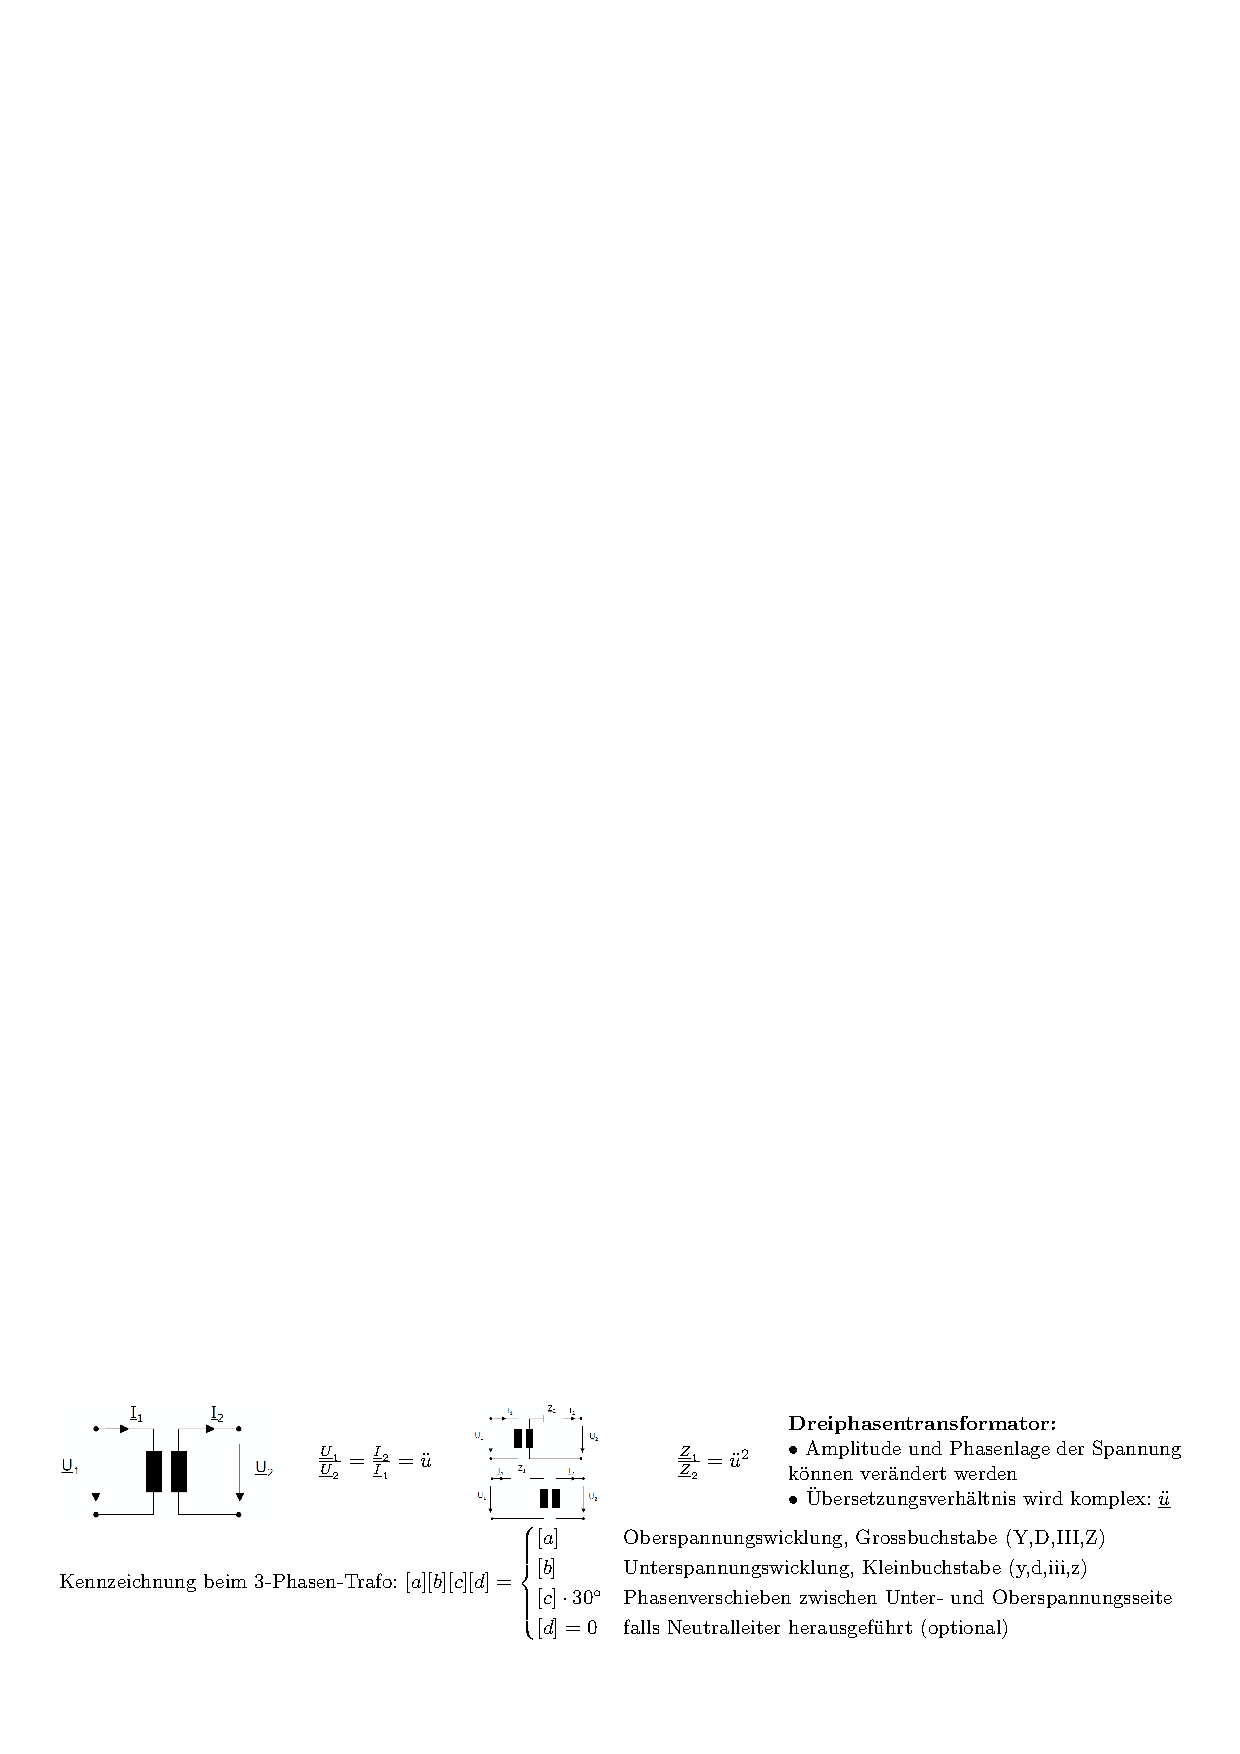
\includegraphics[width=\textwidth]{./images/Trafomodell.pdf}
		ü$_0 = \frac{w_1 \pm \Delta w_1}{w_2} = $ü$_N + \Delta$ü \\
		$X_T = u_K \cdot \frac{U_N^2}{S_{NT}}$
	\subsection{Active power transmission}
		\includegraphics[width=\textwidth]{./images/MOdellierung.pdf}	
		
	\subsection{Frequenzregelung im Verbundnetz}
		grid droop for UCTE: $c_P = \frac{\Delta P / P_N}{\Delta f / f_N}  \approx 0.5; \hspace{1cm}$ Droop: $s = - \frac{\Delta f / f_N}{\Delta P / P_N}; \hspace{1cm}  K_{Regulation} = \frac{\Delta P}{\Delta f} = s^{-1} \frac{P_N}{f_N} \quad [MW/Hz]$ \newline
		
		\textbf{Primärregelung - erste Sekunden (15- 30 s): alle reagieren}\newline
		$\bullet$ dezentrale Regelung  $\bullet$ basiert auf lokaler Frequenzmessung  $\bullet$ Frequenz-Leistungs-Statistik = P-Regler (bleibende Abweichung!)  $\bullet$ findet vollautomatisch und lokal im Turbinenregler des Kraftwerks statt  $\bullet$ Erbringung im gesamten Netzgebiet  $\bullet$ gesamte Netzkennzahl $MW/Hz$ wird auf Länder aufgeteilt  $\bullet$ jedes Land leistet entsprechenden Beitrag (CH $\approx 70~MW$, UCTE $\approx 3000~MW/Hz$)  $\bullet P_P = \Delta f \cdot K_{CH}$ \newline
	
		\textbf{Sekundärregelung - erst Minuten: ausgewählte 'Teamkollegen' übernehmen}\newline
		$\bullet$ basiert auf Messwertsummen der Grenzleitungen, Frequenzabweichungen und dem Korrektursignal Synchronzeit  $\bullet$ PI-Regler  $\bullet$ führt Frequenz zurück auf Sollwert $f_{soll} = f_{old} + \frac{\Delta P_{SR}}{K_{SR}}$  $\bullet$ findet vollautomatisch im zentralen Netzregler der Regelzone statt  $\bullet$ Erbringung durch entsprechende Regelzone  $\bullet$ CH $\approx 400~MW$ \newline
		
		\textbf{Tertiärregelung - nach einigen Minuten: 'Ersatzfahrer' steigt auf}\newline
		
		$\bullet$ Entlastung der Sekundärregelung  $\bullet$ zentral und manuell durchgeführt  $\bullet$ manueller Abruf  $\bullet$ ermöglicht nach einer Störung die neuerliche Optimierung des Kraftwerkeinsatzes  $\bullet$ Dispatcher trifft Entscheidungen  $\bullet P_T = P_{Ausfall} - P_P - P_S$  $\bullet$ CH $\approx +450/-390~MW$ 
		
		
	\subsection{Netzsicherheit und Massnahmen}
	\begin{minipage}[lt]{14cm}
		\textbf{$n-1$-Sicherheit}\newline
		$\bullet$ der Ausfall eines Betriebsmittels darf zu keiner Überlastung eines anderen Betriebsmittels führen  $\bullet$ $n$: ist die aktuelle Anzahl der Betriebsmittel  $\bullet$ nach Ausfall eines Betriebsmittels stehen nur noch $n-1$ Betriebsmittel zu Verfügung  $\bullet$ bei Verletzung der $n-1$-Sicherheit ist noch nichts passiert  $\bullet$ keine $n-1$-Sicherheit = keine Reserve  $\bullet$ Verhinderung Kaskadeneffekt \newline
		
		\textbf{Massnahmen bei Gefährdung der Netzsicherheit} \newline
		$\bullet$ Topologische Massnahmen (Umleiten der Lastflüsse durch Veränderung der Topologie $\Rightarrow$ Änderung der Sammelschienen Konfiguration, Stufen von Transformatoren, Zu-/Abschalten von Leitungen und Trafos, FACTS)  $\bullet$ Produktionsverschiebung (Redispatch $\Rightarrow$ Eingriff in die Produktion = Eingriff in den Markt = unerwünscht)  $\bullet$ Lastabwurf (siehe Abb. \ref{Grid:freq})
	\end{minipage}
	\begin{minipage}[rt]{5cm}
		\hfill
		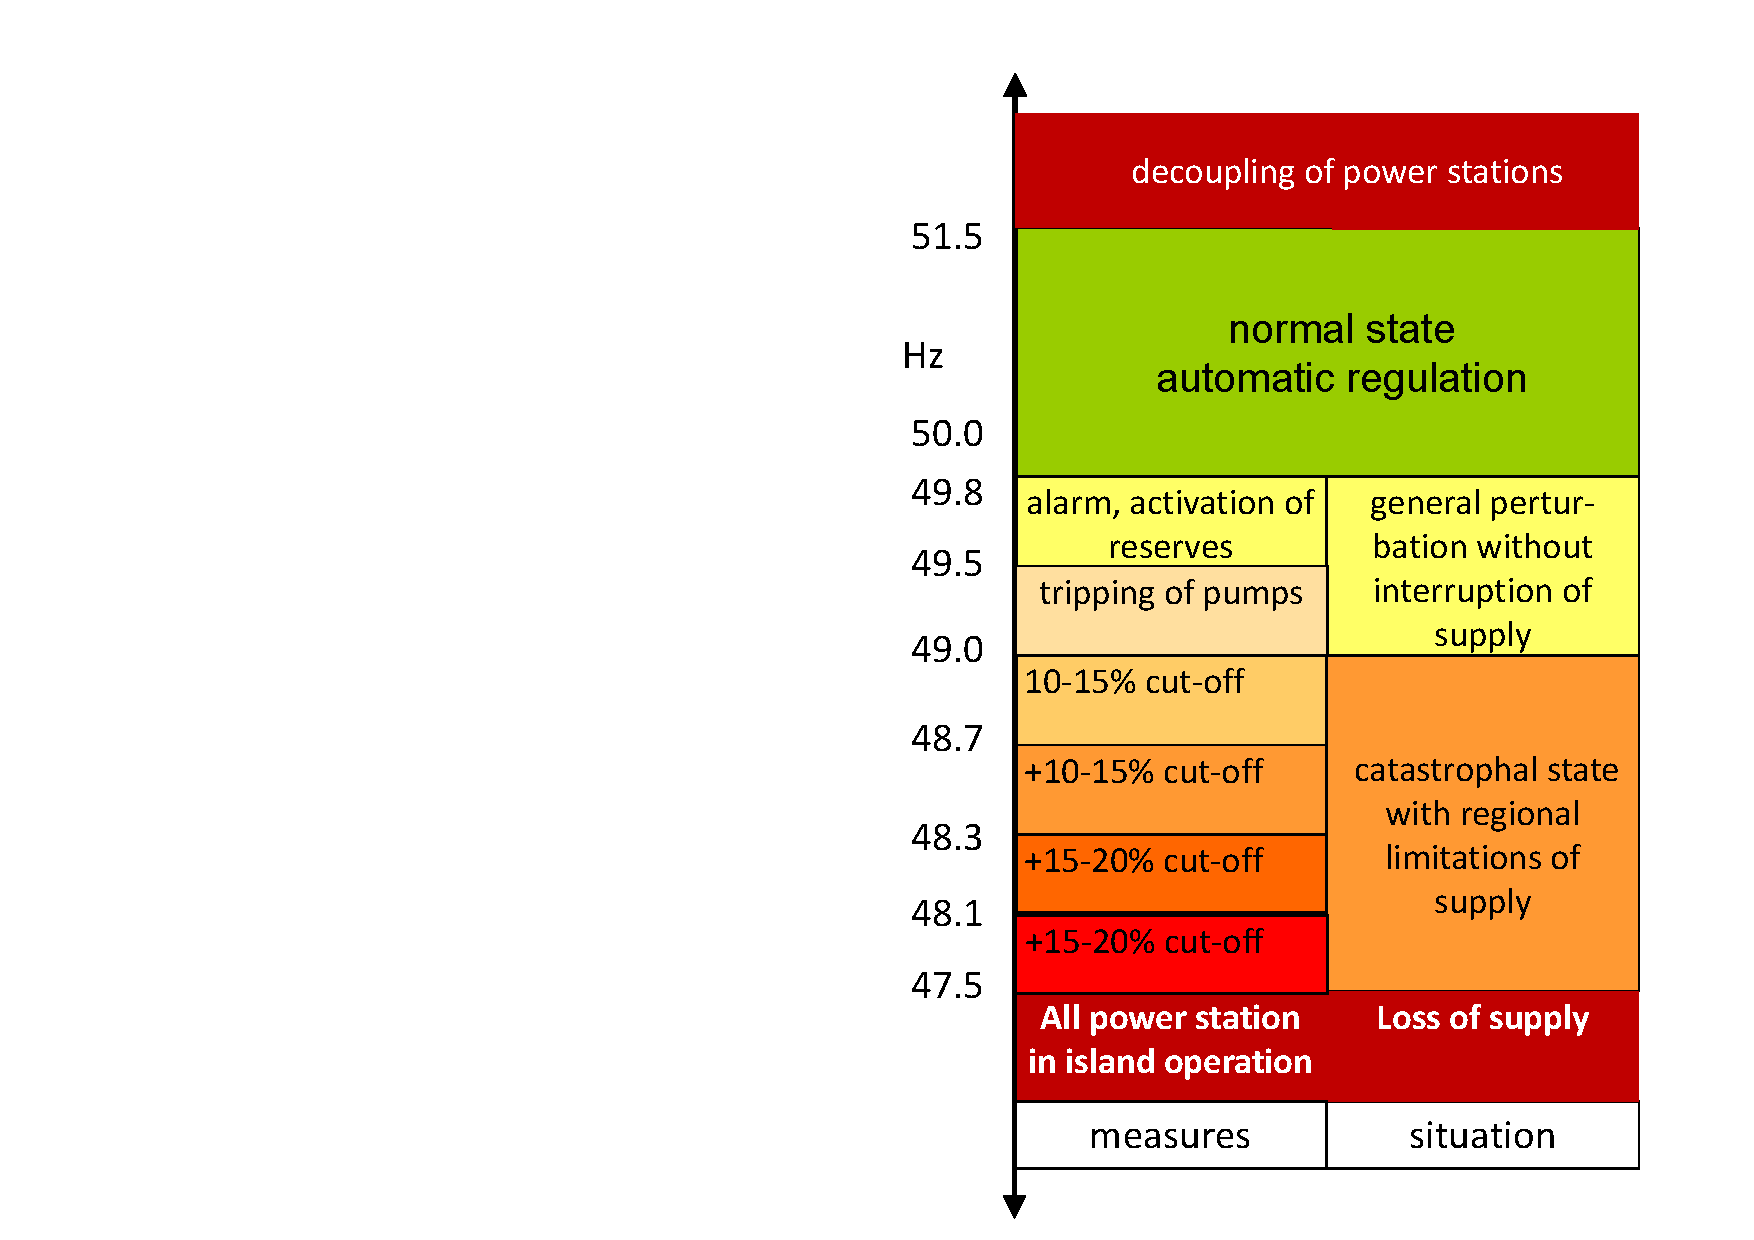
\includegraphics[width=0.75\textwidth]{./images/frequenz.pdf}
		\label{Grid:freq}		
	\end{minipage}
	
	\subsection{Voltage quality}
	\begin{multicols}{2}


		{\footnotesize 	\begin{itemize}
		\setlength{\itemsep}{0pt}
		\item \textbf{voltage}: sinusoidal as possible, amplitude and frequency in rated values
		\item \textbf{harmonics}: reduced durability of capacitors and motors \\$\rightarrow THD_u = \frac{\sqrt{\sum_{i = 2}^{40} U_i^2}}{U_1} \leq 8 \% \hspace{1cm} THD_i = \frac{\sqrt{\sum_{x = 2}^{50} I_x^2}}{I_A} \leq \frac{20}{1000} \cdot \sqrt{\frac{S_{K}}{S_A}}  $
		\item \textbf{flickere (periodic voltage oscillation)}: oscillation of the light density
		\item \textbf{unbalance}: thermal losses/vibrations in el. machines
		\item \textbf{(commutation-)notches}: disturbance of process controls, crash
		\end{itemize}}
	
		{\footnotesize 	\begin{tabular}{|c|c|c|c|}
		\hline \textbf{Characteristic of} &\textbf{Values/} & \textbf{mean} & \textbf{observation}\\
		 \textbf{the voltage} & \textbf{tolerance} & x & \textbf{time} \\ 
		\hline \textbf{Frequency} & $50~Hz; \pm 1\%$ & 10 s & 1 year \\ 
		\hline \textbf{Voltage magnitude} & $\pm 10\% U_N$ & 10 min & 1 week \\ 
		\hline \textbf{longterm flicker} & $P_{lt} = 1$ & 2h & 1 week \\ 
		\hline \textbf{Harmonics} & $THD \leq 8\%$ & 10 min & 1 week \\ 
		\hline \textbf{Unbalance} & $U_2/U_1 < 2\%$ & 10 min & 1 week \\ 
		\hline 
		\end{tabular} }
	\end{multicols}
	
	\subsection{HVDC}
	\begin{minipage}[lt]{13cm}
		{\footnotesize 	\begin{tabular}{|c|c|c|c|}
		\hline  & \textbf{HVAC} & \textbf{HVDC} & \textbf{HVDC/HVAC} \\ 
		\hline Nominal voltage for & $U_\lambda = \frac{U_{Iso}}{\sqrt{2}}$ & $U_{DC} = U_{Iso}$& $\frac{U_{DC}}{U_{AC}} = \frac{\sqrt{2}}{\sqrt{3}}$\\
		the same isolation & $\Rightarrow U_{AC} = \frac{\sqrt{3}}{\sqrt{2}} \cdot U_{Iso}$ & 
		 &  \\ 
		\hline Transmission power & $S_{AC} = \sqrt{3} \cdot U_{AC} \cdot I_{AC}$ & $S_{DC} = 2 \cdot U_{DC} \cdot I_{DC}$ & $\frac{2 \sqrt{2} \cdot I_{DC}}{3 \cdot I_{AC}}$ \\ 
		\hline Transmission losses & $P_{VAC} = 3 \cdot I_{AC}^2 \cdot R_{AC}$ & $P_{VDC} = 2 \cdot R_{DC} \cdot I_{DC}^2$ & $\frac{9 \cdot R_{DC}}{3 \cdot 4\cdot R_{AC}} \approx \frac{3}{4}$ \\ 
		\hline Material (ropes) & $V_{AC} = 3 \cdot A_{AC} \cdot l$ & $V_{DC} = 2 \cdot A_{DC} \cdot l = \frac{3}{2} \cdot A_{AC} \cdot l$ & 0.5 \\ 
		\hline 
		\end{tabular} }
	\end{minipage}
	\begin{minipage}[rt] {6cm}
		$U_{DC \alpha} = 1.35 \cdot U_\Delta \cdot \cos \alpha$ \\
		$\alpha:$ firing angle\\
		$U_{DC} = \frac{1}{\pi/3} \int_{-\pi/6}^{\pi/6} \sqrt{2}U \cos(\omega t) d(\omega t)$\\
		Converter: $U_{AC\Delta} = \frac{U_{DC}}{1.4 \cdot 2}$\\
		$D_{w\Delta Y} = \frac{U_1 \cdot \sqrt{3}}{U_2} \hspace{1cm} D_{w\Delta\Delta} = \frac{U_1}{U_2}$\\
		$D_{wY\Delta} = \frac{U_1}{U_2  \cdot \sqrt{3}} \hspace{1cm} D_{wYY} = \frac{U_1}{U_2}$
	\end{minipage}
	
	\begin{multicols}{2}
		\subsection{Starpoint (phase fault between $3N$)}
		\begin{itemize}
			\setlength{\itemsep}{0pt}
			\item \textbf{rigid earthing}: LV, EHV (and MV when meshed), fast identification of fault, after a longer time for all, $I_K = \frac{U_{3N}}{Z_K} = \frac{U_N/\sqrt{3}}{Z_K}$
			\item \textbf{isolated}: MV, $\underline{I}_F = \frac{\underline{U}_{13}}{-jX_{CE}} + \frac{\underline{U}_{23}}{-jX_{CE}} = \frac{\sqrt{3}U_N}{X_{CE}}$
			\item \textbf{compensated}: MV after a certain time or with enough cables, $\frac{U_{3N}}{X_D} = \frac{\sqrt{3} U_N}{X_{CE}} \Rightarrow X_D = \frac{X_{CE}}{3} \Rightarrow L = \frac{X_D}{\omega}$ 
		\end{itemize}
		
		\subsection{Short-circuit calculation}
		$I_k'' = \frac{c \cdot U_N}{\sqrt{3} \cdot Z_k}$\\
		$\underline{S}_k'' = \sqrt{3} \cdot \underline{U}_N \cdot \underline{I}_k''^*$ \\
		$\underline{Z}_k = \frac{c \cdot \underline{U}_N^2}{\underline{S}_k''^*}$\\ 
		simplified: $c = 1.1$ (siehe Tabelle \ref{tab:SM}) \\
		Single Phase Load: $S_A = k_u (\approx 0.7 \%)\cdot S_k$

	\end{multicols}
\section{Batteries}

\begin{multicols}{2}
{\small 	\textbf{Pb Batteries} 
	\begin{equation*}
		Pb + PbO_2 + 2H_2SO_4 \Leftrightarrow 2PbSO_4 + 2H_2O
	\end{equation*}
	
	\begin{itemize}
		\setlength{\itemsep}{0pt}
		\item[+] Low price due to high number of pieces
		\item[+] Available in many different types
		\item[+] Well recyclable
		\item[-] Slight specific energy
		\item[-] Not allowed for deep discharging
		\item[-] Low lifespan and temp. sensitive
	\end{itemize}
	
	\textbf{NiCd}
	\begin{equation*}
		2NiOOH + Cd + 2H_20 \Leftrightarrow 2Ni(OH)_2 + Cd(OH)_2
	\end{equation*}
	
	\begin{itemize}
		\setlength{\itemsep}{0pt}
		\item[+] High power, fast-chargeable (0.1 - 4C)
		\item[+] Low temperature compatibility
		\item[+] High number of cycles (1000 - 4000)
		\item[-] Temperature sensitive
		\item[-] Memory effect
		\item[-] Highly self-discharging rate
	\end{itemize}
	
	\textbf{NiMH}
	\begin{equation*}
		NiOOH + MeH \Leftrightarrow Ni(OH)_2 + Me
	\end{equation*}

	\begin{itemize}
		\setlength{\itemsep}{0pt}
		\item[+] High energy density
		\item[+] Fast chargeable
		\item[+] Low costs and ecological
		\item[-] Low power density
		\item[-] Memory effect
		\item[-] High self-discharging rate
	\end{itemize}
	
	\textbf{Lithium Ion Batteries}
	
	\begin{itemize}
		\setlength{\itemsep}{0pt}
		\item[+] High voltage $U = 3.6~V$
		\item[+] High specific energy density
		\item[+] High discharge current of 10C
		\item[-] low thermal stability
		\item[-] rather expensive
		\item[-] charging is complicated
	\end{itemize}}	
	
\end{multicols}


\begin{multicols}{3}
\subsection{Peukert factor}
	Peukert factor $k$; $1.1 (better) < k < 1.5$: 
	\begin{equation*}
		H_x = H_0 \cdot \left(\frac{H_0}{T_0 \cdot I_x}\right)^{k-1}
	\end{equation*}	
	\begin{equation*}
		I_k \cdot t_e = C
	\end{equation*}
	\\ \\ \\
{\footnotesize 	\begin{tabbing}
		$I_k$: \hspace{0.1cm} \= Peukert corrected discharge current \\
		$t_e$: \> discharge time \\
		$C$: \> constant \\
		$H_x$: \> available capacity \\
		$I_x$: \> applied current \\
		$H_0$: \> manufacturer's capacity value [Ah] \\
		\> corresponding to the discharge time $T_0$ [h]
	\end{tabbing}}


\subsection{ESR}
Take highest ($I_1$) and lowest ($I_2$) current curve and determine corresponding voltage points ($U_{11}$ and $U_{12}$).
\begin{equation*}
	R_{ESR} = \frac{U_{12} - U_{11}}{I_1 - I_2}
\end{equation*}

\end{multicols}

\subsection{Modelling}
\begin{minipage}[lt]{7cm}
	\centering
	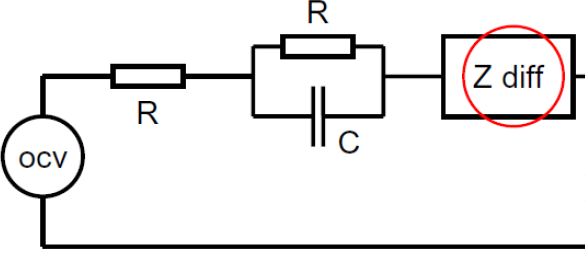
\includegraphics[width=0.7\textwidth]{./images/Battery_modelling.png}
\end{minipage}
\begin{minipage}[rt]{10cm}
	The aging process is simulated with $Z_{diff}$. One possible calculation for this impedance is the so called Warburg impedance (semi-infinite diffusion).
	\begin{equation*}
		Z\left(\omega\right) = \frac{K}{\sqrt{j\omega}} = \frac{K \left(1-j\right)}{\sqrt{2\omega}}
	\end{equation*}
\end{minipage}

\section{SuperCaps}
\begin{minipage}[lt]{10cm}
	{\footnotesize \begin{tabular}[c]{ | p{3cm} | p{6cm} |}
	    	\hline
	    	voltage		  & $\sim 2~V$ \\
	    	\hline
	    	capacity	  & $\sim 3000~F$ \\
	    	\hline
	    	power density & $P' = \frac{U_{SCAPmax} \cdot I}{m} \frac{U_{SCAPmax}^2}{4 \cdot R_s \dot m} \quad m =$ Masse\\
	    	\hline
	    	energy		  & $W' = \frac{1}{2 \cdot m} \cdot C \cdot U_{SCAPmax}^2$ \\
	    	 & $\rightarrow U = \sqrt{\frac{2 \cdot E}{C}}$\\
	    	\hline
	    	efficiency	  & $\eta = \frac{R_L}{R_L + R_S} \rightarrow$ max @$50\%: R_L = R_S$ \\
	    	 & $\eta = \frac{U - R_S \cdot I}{U} = \frac{P - R I^2}{P}$ \\
	    	\hline
	\end{tabular}}
\end{minipage}
\begin{minipage}[rt]{7cm}
	\centering
	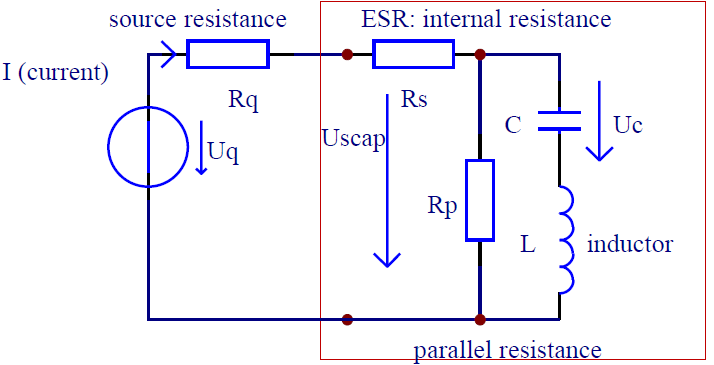
\includegraphics[width=0.9\textwidth]{./images/SCAP_real.png}
	\captionof{figure}{Real model for a SCAP}
\end{minipage}
\begin{figure}[h!]
	\centering
  	\begin{subfigure}[t]{0.49\textwidth}
		\centering
		\adjustbox{width=\textwidth}{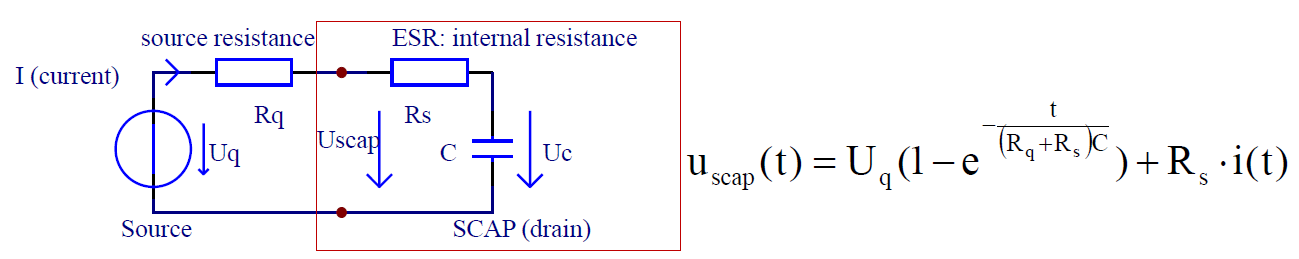
\includegraphics{./images/SCAP_laden.png}}
	   	\caption{charging}
	\end{subfigure}
	\begin{subfigure}[t]{0.49\textwidth}
	 	\centering
	    \adjustbox{width=\textwidth}{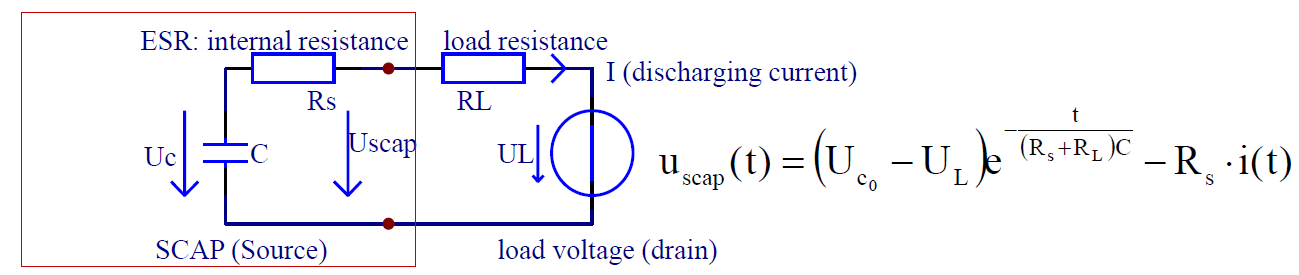
\includegraphics{./images/SCAP_entladen.png}}
	    \caption{discharging}
	\end{subfigure}
	\caption{Simplified model for a SCAP}
\end{figure}


\section{Windkraft}
\begin{minipage}[lt]{10cm}
	max. Windleistung: $P_{max} = \frac{dW}{dt} = \frac{1}{2} \cdot \rho \cdot A \cdot v_1^3$\\
	Leistungsbeiwert: $c_P = \frac{P_W}{P_{max}} = 0.3 \dots \frac{16}{27}$\\
	Windturbinenleistung: $P_W = c_P \cdot P_{max} = c_P \cdot \frac{1}{2} \cdot \rho \cdot A \cdot v_1^3$\\
	Dichte Luft: $\rho_{Luft} \approx 1.29~kg/m^3$
\end{minipage}
\begin{minipage}[rt]{5cm}
	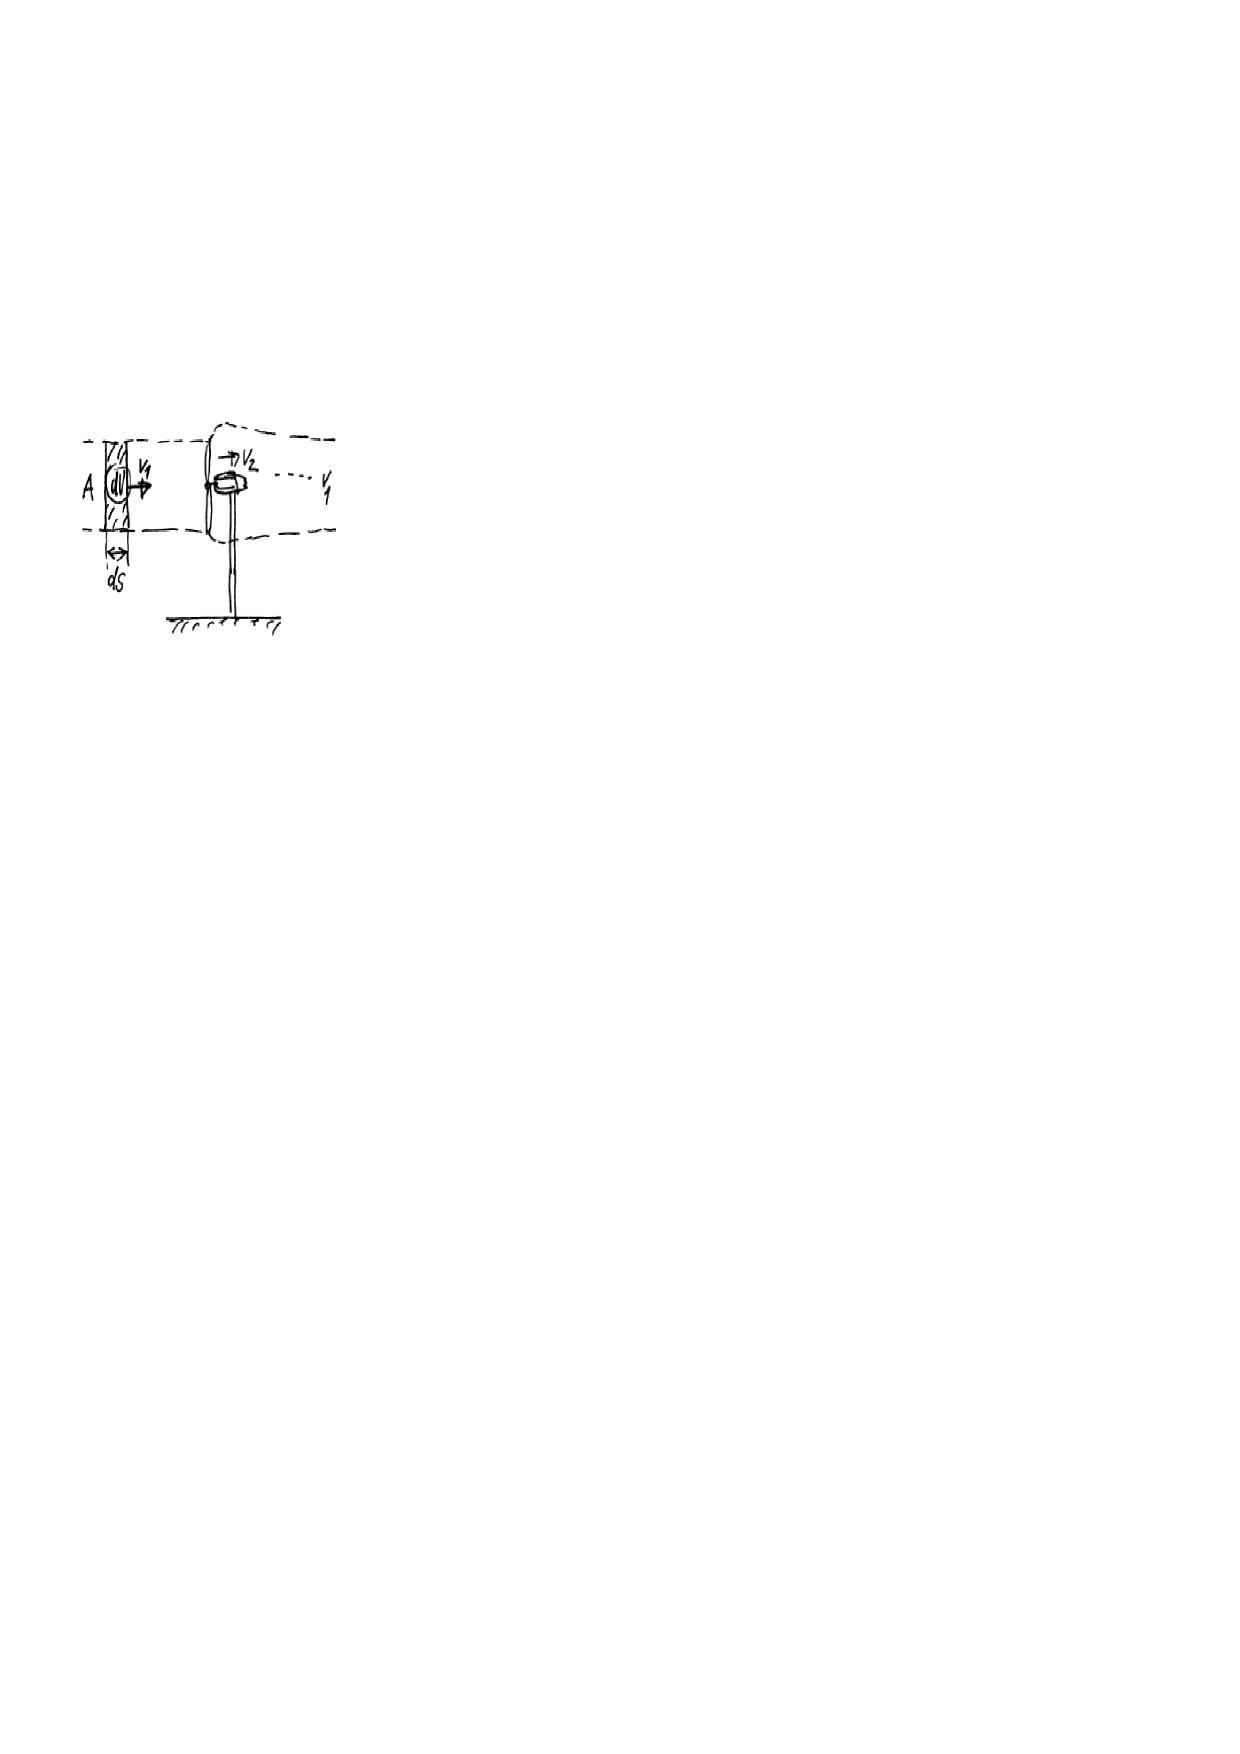
\includegraphics[width=0.7\textwidth]{./images/Wind.pdf}
\end{minipage}
	
		

\end{document}
